% This is LLNCS.DOC the documentation file of
% the LaTeX2e class from Springer-Verlag
% for Lecture Notes in Computer Science, version 2.4
\documentclass{llncs}
\usepackage{llncsdoc}

\usepackage[T1]{fontenc}
\usepackage[latin1]{inputenc}
\usepackage[table, svgnames]{xcolor} 
\usepackage{color} 
\usepackage{url}
\usepackage{graphicx, array, blindtext}
\usepackage[tight,footnotesize]{subfigure}
\usepackage{mdframed}
\usepackage{latexsym}
\usepackage{boxedminipage}
\usepackage{ amssymb }
\usepackage[normalem]{ulem}
\usepackage{flushend}

\usepackage{ocgx}
\usepackage{tikz}
\usetikzlibrary{ocgx}

\usepackage{blindtext}
\usepackage{scrextend}
\usepackage{multirow}
\addtokomafont{labelinglabel}{\ttfamily}

\setlength\floatsep{1\baselineskip plus 3pt minus 2pt}
\setlength\textfloatsep{1\baselineskip plus 3pt minus 2pt}
\setlength\intextsep{1\baselineskip plus 3pt minus 2 pt}
%
\begin{document}

\begin{center}

\LARGE \textbf{Why are program analysis tools difficult to understand?} \\
\Large A tool (mis)communication theory and adaptive approach for supporting developers during tool use \\[2.0em]

\end{center}

\begin{center}
	Brittany Johnson\\[1.0em]
	NC State University \\
	bijohnso@ncsu.edu
	
\end{center}


\vspace{2pt}

\begin{abstract}
	
\end{abstract}

\vfill

%\rule{\textwidth}{1pt}
%\begin{flushleft}
%\large\itshape
%\begin{tabular}{@{}l}
%{\Large\upshape\bfseries Springer}\\[8pt]
%Berlin\enspace Heidelberg\enspace New\kern0.1em York\\[5pt]
%Barcelona\enspace Budapest\enspace Hong\kern0.2em Kong\\[5pt]
%London\enspace Milan\enspace Paris\enspace\\[5pt]
%Santa\kern0.2em Clara\enspace Singapore\enspace Tokyo
%\end{tabular}
%\end{flushleft}


%
%{\tt svserv@vax.ntp.springer.de}\hfil first try the \verb|help|
%command.
%



%
%\newpage
%\tableofcontents
%\newpage
%

\section{Introduction}


\fbox{
	\parbox{\textwidth}{I propose program analysis \emph{tool use} is a form of \emph{communication} and \emph{inability to resolve} notifications is a result of \emph{miscommunication}, therefore we can improve tool design by adopting a theory similar to \emph{constructivism} where tools can \emph{approximate} individual developer's \emph{conceptual knowledge} to adapt notifications, leading to \emph{reduced time and context-switching} required for developers to understand and resolve tool notifications.		}
	}
% TODO make sure later it's obvious how (and why) will assess time and context-switching
%


\section{Research Significance}

\subsection*{Motivating Example}
% merge motivating examples from icse and fse papers into one big example (make sure detailed but say what I mean!)

\begin{figure} [ht]
	\centering
	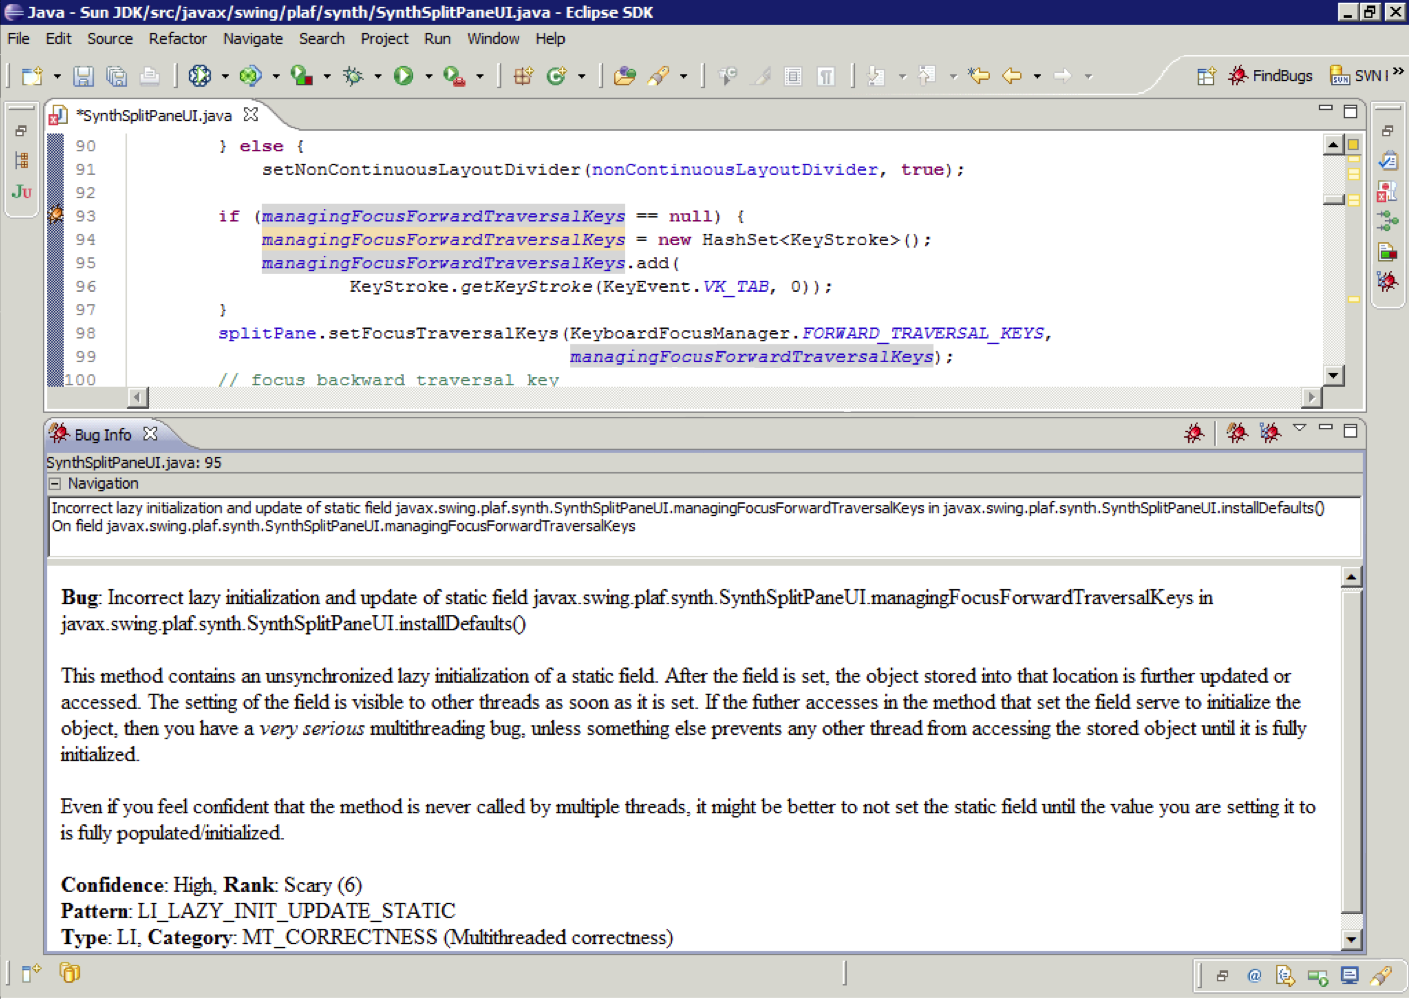
\includegraphics[width=\textwidth]{figs/eclipse.png}
	\caption{Findbugs notification in the Eclipse IDE concerning multi-threading.}
	\label{fig:eclipse}
\end{figure} 

Valerie is a software developer at a start-up company. She primarily writes Java code, though she did not learn to program in Java, and uses the Eclipse Integrated Development Environment (IDE). In her spare time, she builds her knowledge of Java programming concepts by contributing to open source software and using tools that provide feedback about the code she writes. While modifying code in the Sun JDK source code repository, she contributes code that results in the notification shown in Figure~\ref{fig:eclipse}. She has experience using FindBugs, so she is familiar with some of the ways FindBugs communicates. For example, she knows that an orange bug icon indicates a \textit{scary} bug and that by clicking the bug icon she can gain access to more information about the bug.

As she explores the information provided by FindBugs, she realizes that despite her experience with FindBugs, she is having difficulty determining how to resolve the notification. She first attempts to use what knowledge she does have regarding multi-threading, which she accrued from struggling with and resolving compiler synchronization warnings, to better understand the problem. 
% TODO not clear what "the problem" is - be specific
However, she is unfamiliar with the concept central to the notification in Figure~\ref{fig:eclipse} (lazy initialization). Though the notification tells her that the problem relates to multi-threading, she is unable to make a connection between her knowledge regarding multi-threading and the message FindBugs is attempting to communicate and therefore cannot resolve the notification without outside help. As done previously with compiler synchronization notifications, she toggles between the web and her IDE to understand and resolve the notification.

% TODO compiler synchronization notification??

\begin{figure} 
	\centering
	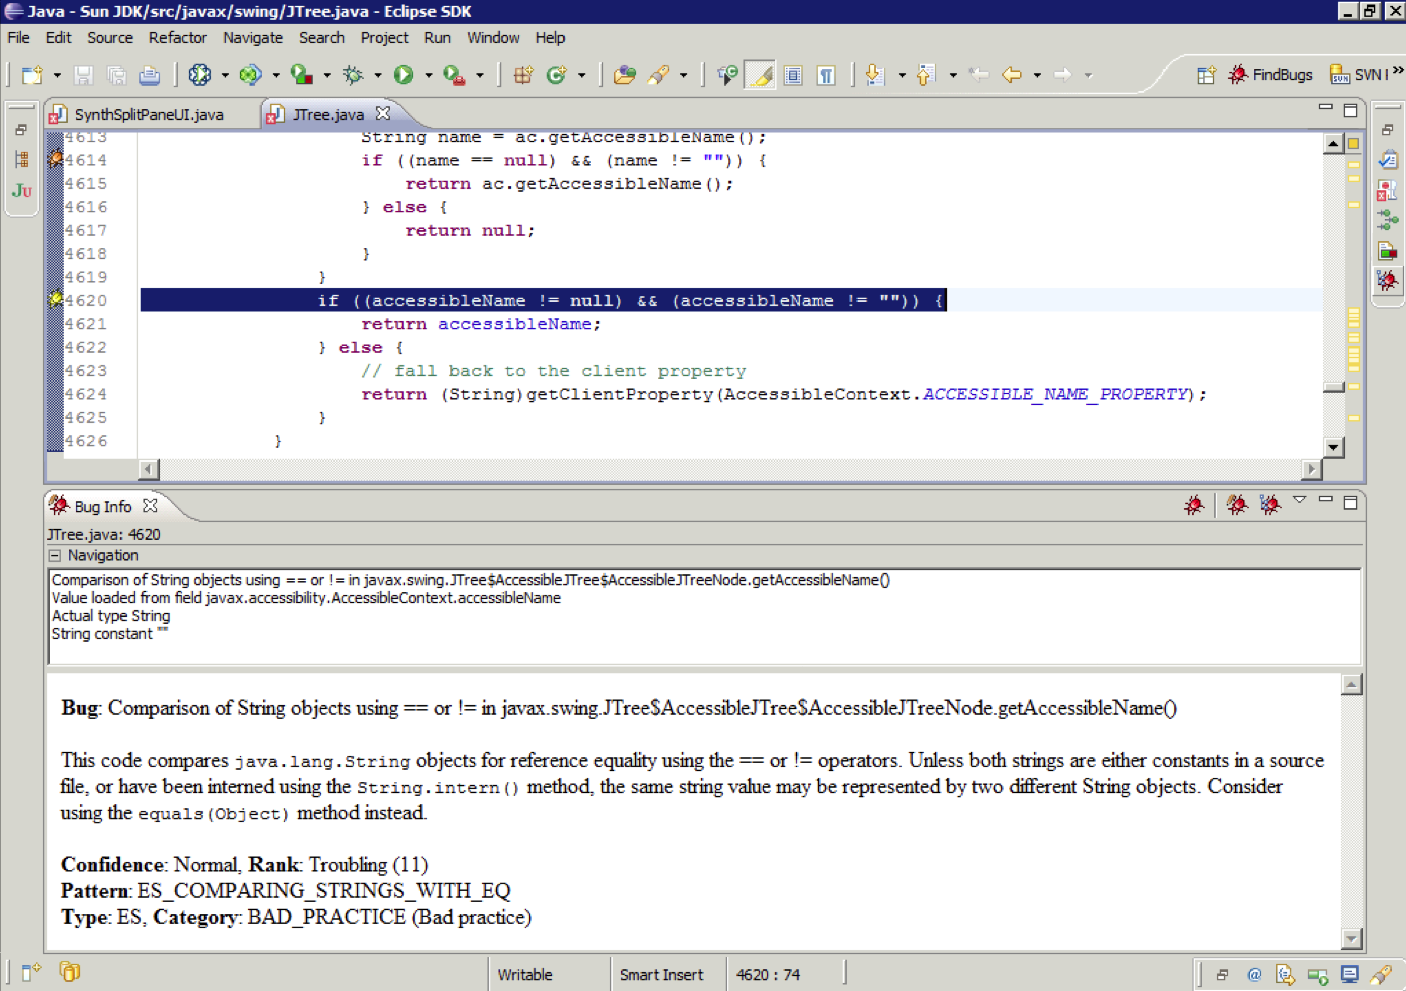
\includegraphics[width=\textwidth]{figs/eclipse-2.png}
	\caption{Findbugs notification in the Eclipse IDE on checking string equality.}
	\label{fig:eclipse2}
\end{figure}

Although Valerie's goal when using tools like FindBugs is to find and resolve defects, which requires the ability to interpret the notifications provided by the tools, a secondary goal is to learn more about Java programming concepts. She found, however, that some notifications are better at communicating problems while contributing to knowledge than others. For example, when first learning how to work with strings in Java, Valerie encountered the notification in Figure~\ref{fig:eclipse2}. The first time she encountered the problem she was able to understand and resolve the notification. Looking back, she realizes this was because the notification in Figure~\ref{fig:eclipse2} filled in gaps in her own knowledge of the concept by informing her \emph{why} what she was doing was wrong and \emph{how} she can fix it.

Because the tools Valerie uses have no notion of what she does and does not know, some notifications communicate in a way that she is able to understand the problem, while others are not, leading to  miscommunication. In the following sections, I will discuss research that explores challenges like those encountered by Valerie and motivate research for developing techniques, frameworks, and tools that mitigate these challenges.

\begin{figure} [ht]
	\centering
	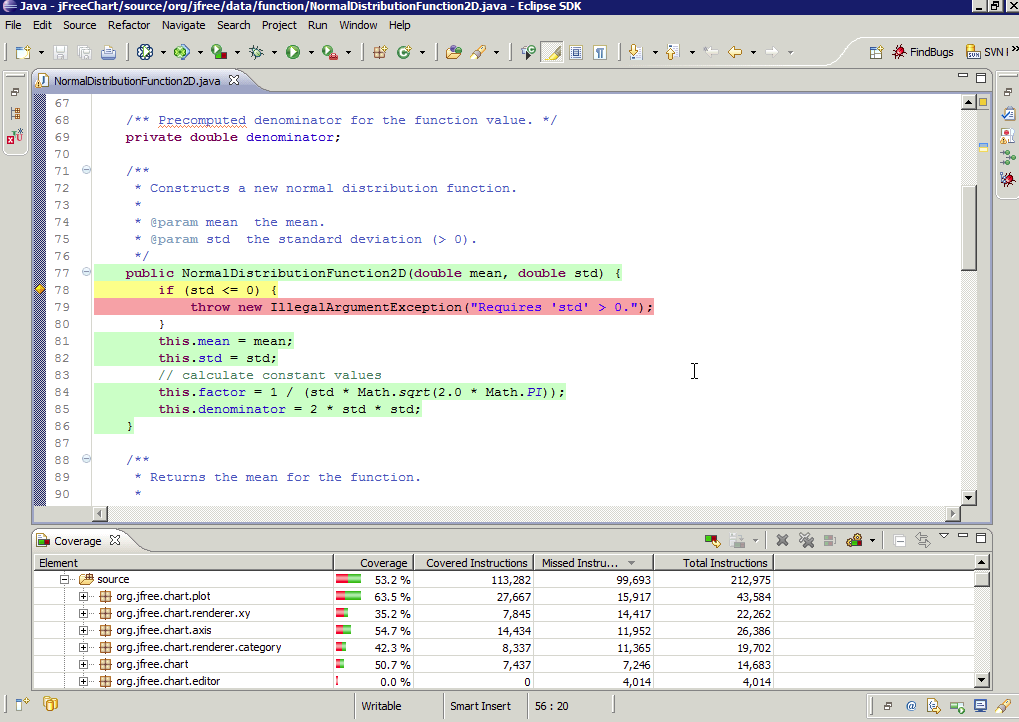
\includegraphics[width=\textwidth]{figs/eclemma.png}
	\caption{EclEmma notifications in the Eclipse IDE.}
	\label{fig:ecl}
\end{figure}

\subsection{What are program analysis tools?}
Program analysis tools are designed to aide developers when developing software by automating the writing, analysis, and modification of source code.
Often, program analysis is discussed as synonymous with static analysis~\cite{nielson2015principles}. 
For the purpose of my research, I define a program analysis tool as a recommendation system that performs program analysis, whether it be static or dynamic analysis, and provides information regarding the source code being analyzed~\cite{robillard2014recommendation}.
Examples of program analysis tools include, but are not limited to, static code analyzers, code coverage tools, code smell detectors, and refactoring tools~\cite{adolph2011using,Murphy-Hill:2010:Ambient,ge2012reconciling}.
In the following sections, I will define and discuss static analysis and dynamic analysis tools separately; the reader should note that although we discuss static and dynamic analysis separately, it is not uncommon to find program analysis tools that combine static and dynamic analysis~\cite{ernst2003static}.                                                

\subsubsection{Static Analysis Tools.}

Static analysis tools are designed to aide developers when developing software by statically analyzing source code, pre-runtime, and providing the developer with feedback about the state of their code~\cite{ernst2003static}.
Typically, static analysis works by examining the current state of the program, predicting how the program may react in that state at runtime, and reporting any information they deem necessary to the developer. Static analyses are often more conservative than dynamic analyses; this is to reduce the potential for false positives, as in most cases static analysis cannot say with 100\% certainty what will happen during run-time. 
Examples of static analysis tools include defect detectors, such as FindBugs, compilers, code smell detectors, and refactoring tools.
% TODO talk about what static analysis can do/find to motivate further

Let's use the example of FindBugs,\footnote{http://findbugs.sourceforge.net/factSheet.html} an open source static analysis tool, to better understand how static analysis tools work. FindBugs statically analyzes code to report potential defects. FindBugs determines the potential for defects using \emph{bug patterns}. Bug patterns are code idioms that map to errors, found in Java \emph{bytecode}. Bytecode, in Java, represents the compiled Java class files. Because FindBugs analyzes code without executing it, there is a heightened risk for \emph{false positives}. False positives are defects detected that will never manifest during run-time. When FindBugs finds a potential defect, it alerts the developer using notifications that provide information regarding the defect. I will discuss tool notifications in more detail in Section~\ref{subsec:comm}.


\subsubsection{Dynamic Analysis Tools.}

Dynamic analysis tools are designed to aide developers when developing software by analyzing source code during run-time and providing the developer with feedback about runtime behavior~\cite{ernst2003static}.
Dynamic analysis works by executing the program and then making observations about program execution; because dynamic analysis runs the code, it is typically more precise than static analysis. Though dynamic analysis can produce more precise results in a similar amount of time as static analysis, dynamic analysis execution is less likely to generalize to future executions since it is based on a set of inputs that can, and probably will, change for each execution.
Examples of dynamic analysis tools include testing, code coverage, and profiling tools.

Let's use the example of EclEmma,\footnote{http://eclemma.org/} an open source dynamic code coverage tool, to better understand how dynamic analysis tools work. EclEmma executes source code, using either JUnit test cases or a pre-defined set of inputs, and reports to the user what parts of the code got covered and what parts did not. Because EclEmma executes the source code, it can communicate precisely regarding the flow of the program during run-time. A static code coverage tool could speculate how much of a code base would be covered based on test cases, and possibly even a set of inputs; however, it would require more effort and be more likely to produce false positives than a dynamic code coverage tool. On the down side, the test suites a developer writes may not be characteristic of all possible executions of the program, thereby lowering the generalizability of dynamic analyses.

\subsection{How do tools communicate?}\label{subsec:comm}

One common thread between program analysis tools like FindBugs and EclEmma is that they use \emph{notifications} to communicate with the developer. Figure~\ref{fig:ecl} and Figure~\ref{fig:eclipse} provide examples of tool notifications. A notification, when speaking in terms of program analysis tools, is a combination of visuals and text used to communicate a message to its user; for program analysis tools, the user is the developer.

% TODO: see if I can find a tool that is evenly visual and textual.
Notifications across tools vary; some provide lots of text (like FindBugs), some use primarily visual means of communications (like EclEmma), and some fall in between using equal parts text and visuals to communicate. Notifications can also have different goals, which may influence how developers design notifications. For example, the goal of a FindBugs notification is to explain a potential defect in the developer's source code and, ideally, help the developer make a decision about the defect (i.e. whether and how to resolve). Because FindBugs' goal is to explain, we expect to see textual notifications that provide that explanation.
The goal of EclEmma notifications is to statically show dynamic program behavior and help the developer determine the effectiveness of her test suite. Though EclEmma could use text to communicate code coverage, this takes away the ability to scan the program for areas in most need of attention; therefore, EclEmma uses colors applied directly to the source code to communicate. EclEmma uses other visuals, such as the bar visuals in the Coverage View (Figure~\ref{fig:ecl}) to show coverage on a given package or class.
 % TODO talk about how different parts of notification communicate for each tool; make sure it ties back to goals (defects and test coverage)!

The list of tools and notifications tools use can go on and on, but for the purposes of my research, the general definition I will use for a notification is \emph{a combination of visual and textual information used by a program analysis tool to communicate a message to developers.} Notifications can vary regarding what information and how much detail they provide, however, there are commonalities across tool notifications, which I will discuss next.

\subsection{What are the typical components of a tool notification?}
% based on robilliard book

% recommendation systems break down: somethign to get attention, description
% types of descriptions (text and visual)
% goals of information provided (??)

\subsection{What do tool notifications communicate about?}

% communicate about the state of with source code
The goal of program analysis tool notifications is to communicate to the developer about their source code.
% source code maps to concepts (vann2004, biggerstaff); both human oriented and programming oriented concepts (biggerstaff)
The source code a developers writes is a runnable manifestation of programming-oriented and human-oriented concepts~\cite{van2004concepts,biggerstaff1994program}. 
At the lowest, most fundamental level, are \emph{programming-oriented concepts}, which relate to how the source code maps to programming language concepts.
Programming concepts can be as simple as the means for storing and passing data, such as variables, or as complex as the means for structuring data, such as generics~\cite{jazayeri1997programming}.
At a more abstract level, \emph{human-oriented concepts} relate to the high level goal of the source code, such as ``acquire target'' or ``complete transaction''.

Typically a given notification is associated with only one human-oriented concept.
On the flip side, one notification can communicate about more than one programming-oriented concept. 
Consider the following source code:

\begin{quotation}
	\texttt{There will be some relevant code here :D}
\end{quotation}

The goal, or human-oriented concept, at play is ``write to file''. 
A notification attached to this code is telling the developer something about the code she wrote to ``write to file''.
There are multiple programming-oriented concepts at play, which aligns with the types of notifications the developer may get. 
In the process of writing this code, the developer may get a notification regarding any number of programming-oriented concepts (buffered streams, exception handling); for example, tools like FindBugs, Sonar, and IntelliJ's built-in static analyzers notify developer when they have opened a stream (\texttt{BufferedWriter} in the above example) and there is a possibility the stream that is writing to the file will not close.
A developer may also get a notification regarding exception handling. Here, the developer has written code to catch an \texttt{IOException} if it occurs. However, if she did not implement code to deal with the potential for an \texttt{IOException} she would get a notification communicating the need to do so.

% TODO later, should note that focusing on programming oriented concepts because those generalize and are foundational to developing the abstractions that are human oriented concepts (biggerstaff)

%Notifications communicate about both simple and more complex programming concepts, and often communicate about multiple, typically related, concepts in a given notification. For example, the programming concepts in the notification in Figure~\ref{fig:eclipse} are variables, synchronization, lazy initialization, and multi-threading. The idea of a variable is a simpler concept that can be related to any number of other concepts. Synchronization, lazy initialization, and multi-threading, however, are more complex and relate to each other explicitly and exclusively. Lazy initialization is a specific approach to synchronization, both of which relate to multi-threading. The presence of these concepts narrows the concept of a variable in this notification to a variable in the context of a multi-threaded environment. 

\subsection{Are developers able to interpret tool notifications?}
Despite the possibility provided by program analysis tools for exploration and improvement of source code, research has found that developers often to not use tools like FindBugs~\cite{Ayewah:2008:FindBugs}.
Though research explored tool usage, there was no research that explored the reasons developers have for using the tools they do use and not using the tools they do not use~\cite{Bessey:2010:Coverity,Khoo:2008:PathProjection}.
To answer the question \emph{why do developers not use static analysis tools}, I conducted interactive interviews with 20 professional developers to better understand why they do not use static analysis tools, one type of program analysis tool, when writing code~\cite{johnson2013don}.
Each interactive interview consisted of three parts: 1) an interview regarding past experiences with static analysis tools, 2) an interactive exploration of FindBugs and 3) a participatory design session to discuss suggested tool improvements.

Based on the data from these interviews, the reasons developers do not frequently use static analysis tools are \textbf{Lack of collaborative support}, \textbf{Seemingly unorganized tool output}, \textbf{Poor support for customizations}, and \textbf{Difficult to interpret notifications}. 
Three out of four findings regarding tool use pertain to the notifications tools use and how tools present information to the developer.
Discovering that tool notifications are one of the reasons developers do not use program analysis tools is useful, however, not actionable. The next piece of information needed to make these findings actionable is to discover what about tool notifications make it difficult for developers to interpret their notifications.

\subsection{What challenges do developers encounter when interpreting notifications?}
% interactive interviews (icse) & %session study (fse)
To answer the question \emph{why do developers encounter challenges when interpreting program analysis tool notifications?}, I observed 26 developers with varying backgrounds while they used three different program analysis tools: Eclipse Java compiler, FindBugs, and EclEmma. I presented participants with and asked them to interpret notifications from each of the three tools. 
% TODO need something relevant to cross-tool!
To identify challenges, we examined tool use through the lens of communication theory~\cite{bowman1987modeling}.
Building on an existing model of (mis)communication~\cite{mustajoki2008modelling}, we identified 

% TODO expand here! What did I do/find and how does it relate to communication/miscommunication??



Based on findings from these studies, I identified the following problems with the state-of-the-art in program analysis tool notification design:

\begin{itemize}
	\item Tool notifications can be difficult to sort through and interpret, making them difficult to use.
	\item Many notifications do not effectively and consistently communicate to accommodate individual developer knowledge.
\end{itemize}

\section{A Tool Miscommunication Theory}\label{sec:theory}
%session study (fse)
Based on the challenges participants encounter when interpreting tool notifications, I propose a tool miscommunication theory that can be used to inform the design of program analysis tools.
Experts in qualitative research suggest that rather than presenting a set of disparate findings, qualitative researchers should instead produce an explanatory theory, a ``skeleton or framework that explains why things happen''~\cite{corbin2014basics}. While explicitly putting forward theories is rare in software engineering~\cite{hannay2007systematic}, one example is Lawrance and colleagues' theory of how programmers navigate code during debugging~\cite{lawrance2013programmers}. In the same way that Lawrance and colleagues' build on 
information foraging theory~\cite{pirolli1999information}, my theory builds on communication theory~\cite{bowman1987modeling}.
I summarize my theory as:

\begin{quotation}
	\noindent
	\emph{The challenges developers encounter when interpreting program analysis tool notifications are caused by gaps and mismatches between developer knowledge and how notifications communicate information.}
\end{quotation}

My theory is based on the findings from my most recent study on the challenges developers encounter when interpreting tool notifications. 
I speak about knowledge here and throughout as the culmination of experiences~\cite{johnson1989mental,argote2011organizational}.
Using that definition, a \emph{knowledge gap} occurs when there is a gap between what the developer knows and how the tool communicates; a \emph{knowledge mismatch} occurs when what the developer knows and expects from the tool does not match the notification the tool uses.

Remember Valerie? Though she is a hypothetical developer, the challenges she faced are not hypothetical. Valerie experienced challenges caused by both knowledge gaps (no knowledge regarding lazy initialization) and knowledge mismatches (expecting an explicit connection to synchronization). Based on this theory, I hypothesize that if it was possible for tools to be aware of what developers know and do not know, tools can improve communication by adapting its notifications to the developer.

\section{A Proposed Approach for Modeling Developer Knowledge}
%modeling approach (vlhcc)
In order to adapt tool notifications to a given developer's knowledge, there needs to be some notion of how much the developer knows about the concepts in the notification. I propose that by borrowing from education research and using developer experiences as a concrete representation of knowledge, it is possible to learn and approximately predict developer knowledge of programming concepts.

\subsection{Using Concept Inventories to Assess Concept Knowledge}
% TODO read through and revise as needed! 
To create any kind of model, I need a dependent variable and one or more independent variables that could be used to predict the value of the dependent variable. Since I propose models that predict knowledge, my dependent variable has to be some measure of developer concept knowledge.
Borrowing from existing computer science education research, I developed concept inventories for knowledge assessment. Traditionally, concept inventories are used to  assess conceptual knowledge and identify misconceptions; in Computer Science, the target audience is typically CS1 students~\cite{tew2010developing,kaczmarczyk2010identifying}. I will use concept inventories to assess what any developer knows, rather than what CS1 programmers do not know.

I need to assess knowledge with a wide range of developers outside of academia, therefore I could not borrow directly from research that creates concept inventories for novice academic programming concept knowledge assessment~\cite{tew2010assessing}. I combined existing concept inventory research with examinations using Bloom's Taxonomy~\cite{tew2010developing,nelson1967testing,scott2003bloom}. By using Bloom's Taxonomy to inform question creation, I can increase assurance that my questions exhaustively assess understanding. The current inventory has 10 questions, each worth 1 point, that effectively assess knowledge and represent ground truth conceptual knowledge. The final, validated process I have developed for creating general programming concept inventories is as follows:

\vspace{0.5em}
\noindent\textbf{Define Conceptual Content for Test Specification.} I used sources such as Oracle Documentation and Tutorials to come up with the relevant conceptual content. A test specification is a way of formally outlining what will be on the test without having to write the questions~\cite{tew2010developing}. 

\vspace{0.5em}

\noindent\textbf{Build Bank of Test Questions.} This step is where Bloom's Taxonomy becomes important. Without using Bloom's Taxonomy, I could create a group of questions that potentially assess the same level of understanding. Therefore, I came up with at least 1 question for each level of Bloom's taxonomy, based on my test specification, using examples found in ~\cite{nelson1967testing} and ~\cite{thompson2008bloom}.  

\vspace*{0.5em}

\noindent\textbf{Pilot Questions.} I piloted my initial set of questions with 11 developers and students at NC State University. I did another pilot once I established validity and reliability, the next step.

\vspace*{0.5em}

\noindent \textbf{Establish Validity and Reliability.} To validate my concept inventory, I conducted item analysis~\cite{gorsuch1997exploratory}. The purpose of item analysis is to determine how effective your test, and the items on it, are. The primary goal in the scope of my research was the determine which questions may be considered too easy, too hard, or not fair. From the item analysis, I was able to remove 1 question that, according to my analyses, was not effective.


I discuss the process that led to this final set of steps when I related study in Section~\ref{subsec:s3}.

\subsection{Using Public Git Repositories to Predict Concept Knowledge}
Research suggests that knowledge is often accumulated and organized based on our own relevant experiences~\cite{johnson1989mental,argote2011organizational}. As a developer, many experiences are focused on writing source code; writing software is also perhaps one of the most concrete actions that can be labeled as an experience for a developer. Therefore, I used \emph{concept-specific source code} to determine independent variables for my models. I define concept-specific code is code that maps to a given programming concepts; an example of multi-threading-specific code is \texttt{synchronized(variable)}, where the developer has written code that synchronizes variables for multi-threaded execution.
I built a Java source code analyzer that analyzes code bases for concept-specific code.

To accurately create models, I need to be able to attribute code changes to a specific developer; this is coupled with developer--dependent scores from the concept inventories to create and evaluate the models. Analyzing static code can tell me the presence of conceptually relevant code patterns, such as synchronization or generics usage. However, it can not tell me who contributed that code which is important when trying to build models that can accurately predict individual knowledge. 
Therefore, I propose using version control to automate and ease the process of assigning code contributions to a given developer. 
Version control is also useful for determining how recently a developer has made concept-specific code contributions, which I found can be an important factor when using experience as a proxy for knowledge~\cite{johnson2015bespoke}. % TODO cite vlhcc here if accepted!
I will discuss my approach in more detail in Section~\ref{sec:eval}.
Given the possibility of modeling conceptual knowledge, the next step is to assess the use of these models to determine appropriate feedback to give to the developer in a given notification.


\section{A Proposed Approach for Knowledge-Based Notifications}
% bespoke paper (focused on notifications - fse)
% TODO proof-read and integrate with the rest of paper
Program analysis tools could improve the ability to communicate with developers by aligning notifications with the experience and knowledge of the developer using the tool.
For example, FindBugs provides the following notification:

\vspace*{-1ex}
\begin{quotation}
	\noindent \small{
		This call to a generic collection method passes an argument while compile type Object where a specific type from the generic type parameters is expected. Thus, neither the standard Java type system nor static analysis can provide useful information on whether the object being passed as a parameter is of an appropriate type.}
\end{quotation}
\vspace*{-1ex}

\noindent
A developer who is less familiar with concepts related to generic types might find this notification difficult to understand. 
In contrast, a developer who is very familiar with these concepts might find this notification too verbose or even distracting.

A tool that has access to models that can predict what a developer knows about programming concepts could adapt the notification to the developer looking at it.
To continue the above example, if a developer knows little about the concept of generic types, the message would be more verbose, perhaps providing links to 
relevant on-line material or example solutions.
If a developer knows all the relevant concepts well, the notification could instead simply say ``unchecked generic type,'' and point her to where in the code the generic type parameters are expected.

Like the other examples, the code that the developer has written is a useful source of data for hints about a developer's knowledge of a concept.
For the generic type notification, this includes usage of generics where a generic type parameter is specified and usage of generic objects.
Another source would be notifications she has already resolved; if the developer has resolved notifications of the same kind or notifications that involve the same concepts,
the developer likely has some knowledge of the underlying concepts.

I have outlined my proposed research; next I will outline the studies, experiments, and evaluations I have and will complete for my dissertation research.

\section{Experiments \& Evaluations}\label{sec:eval}
% TODO think about RQs for each
% why don't study (completed)
\subsection{Why don't developers use static analysis tools to find bugs? [Reasons]}\label{subsec:s1}

\subsubsection{Study rationale.} Static analysis tools provide a means for analyzing code without having to run
the code, helping ensure higher quality software throughout the development process. There are a variety of ways to perform automatic static
analyses~\cite{Gegick:2007:AutomatedAnalysis}, including at the developer's request, continuously while creating the software in a development
environment, and just before the software is committed to a version control system. The tool may allow the developer to configure what kinds of bugs it
finds, and sometimes even define new bug patterns. Static analysis tools use well-defined programming rules to find defects early in the development process, when they
are cheap to fix~\cite{Ayewah:2008:FindBugs}. For example, there are static analysis tools that can alert developers to synchronization issues which can
lead to unsafe thread interactions. Developers have been able to eliminate many defects that were previously overlooked at large companies~\cite{Ayewah:2010:GFF} using the warnings produced
by static analysis tools. 
Despite the benefits of using static analysis tools to find bugs, consistent usage of these tools is not very frequent~\cite{Ayewah:2008:FindBugs}. 
There have been studies to investigate ways of improving static analysis tools. However, none look at what the tools do or can do for a developer, what features
developers use, what could be improved \emph{and} why~\cite{Bessey:2010:Coverity,Khoo:2008:PathProjection}. 

\subsubsection{Research questions.}
\begin{labeling}{questions}
	\item [RQ1] What reasons do developers have for using or not using static analysis tools to find bugs?
	\item [RQ2] How well do current static analysis tools fit into the workflows of developers? I define a workflow as the steps a developer takes when writing, inspecting and modifying their code.
	\item [RQ3] What improvements do developers want to see made to static analysis tools?
\end{labeling}

\subsubsection{Participants.}


\subsubsection{Methodology.}
To answer my research questions, I used semi-structured interviews. Each semi-structured interview consisted of three parts: \textit{Question and  Short Response}, \textit{Interactive Interview}, and \textit{Participatory Design}. Once completed, I transcribed and coded each interview. Here I describe each part of the interview and my coding process.

\vspace{0.5em}
\noindent\textit{Question and Short Response.} During the Question and Short Response portion of the interview, we asked developers questions related to their general usage, understanding, and opinion of static analysis tools in order to answer RQ1.
Some of the questions asked include:
\begin{itemize}
	\item Can you tell us about your first experience with a static analysis tool?
	\item Can you remember anything that stood out about this experience as easy or difficult?
	\item Have you ever used a static analysis tool in a team setting? Was it beneficial and why?
	\item Have you ever consciously avoided using a static analysis tool? Why or why not?
	\item What in your opinion are the critical characteristics of a good static analysis tool?
\end{itemize}

\vspace{0.5em}
\noindent\textit{Interactive Interview.}
The goal behind an interactive interview is to be able to observe developers actually using a static analysis tool. This allowed me to get more detailed information as to how developers are using their tools. I  used information obtained during this portion of the interview to answer RQ1 and RQ2. I asked participants to explain what they are doing out loud~\cite{Lewis:1982:ThinkAloudProtocol} so I could get a better understanding of their workflow and thought process as they used the tool. Practice interviews before this study revealed that using the interactive interview portion produced more detailed information regarding when and how developers use their static analysis tools~\cite{Johnson:2012:PreFFSAT}.

Some of the questions asked during the interactive interview include:
\begin{itemize}
	\item Now that you have run your tool and gotten your feedback, what is your next move(s)?
	\item Do you configure the settings of your tool from default? If so, how?
	\item Does this static analysis tool aid in assessing what to do about a warning?
	\item Do you feel that ``quick fixes'' or code suggestions would be helpful if they were available?\footnote{Participants were only asked about quick fixes and code suggestions being useful when they mentioned, either during the Question and Answer or Interactive Interview, that they either a) find quick fixes useful, b) felt that the tool should be more helpful or c) did not understand how to fix the defect we presented them with. }
\end{itemize}

For confidentiality reasons, not all participants could use their own workstation for this part of the interview. For those who could not, I provided 6 open source projects in Java, such as log4j~\cite{log4j} and Ant~\cite{ANT}, and asked each participant to run FindBugs on one of them.  I chose FindBugs because it is one of the most popular and mature static analysis tools for Eclipse. Due to technical difficulties, the remote interviews were not able to fully experience the ``interactive'' portion. I gave each remote participant a scenario of static analysis tool usage and asked them to, first, explain their thought process in walking through that particular scenario. I then asked the same questions as I would have asked if they had been local.

\vspace{0.5em}
\noindent\textit{Participatory Design.}
I used the last part of the interview to solicit participant design suggestions for improving static analysis tools. We utilized a concept called participatory design~\cite{Spinuzzi:2005:Participatory}, which involves
getting stakeholders (in this case, our participants) involved in the design process by allowing them to show what they want instead of saying it. To promote creativity, I gave each participant a blank sheet of paper and asked them to show me what they wanted their tool to look like and how it should work~\cite{Johnson:2012:PreFFSAT}. It was not mandatory for participants to draw something, but 6 of them did. The other participants gave verbal descriptions of tool features they desired.

\vspace{0.5em}
\noindent\textit{Coding Interview Responses.}
After completing the interviews, I manually transcribed each interview. Then, I \textit{coded} the final transcripts. Coding is a process that is meant to make referencing transcriptions quicker and
easier~\cite{Gordon:1998:Coding}. I used Gordon's basic steps to code the interviews. Before coding an interview, ``coding categories'' need to be defined. These should be general enough for relevant information to be grouped together but detailed enough that a concrete example only falls under one category. Because of this, it is possible to have ``emergent'' categories that may need to be defined after reading the transcriptions. The final set of coding categories, along with an example quote for each, are as follows: 

\begin{description}
	\item[Tool Output] -- Anything related to the output produced by the tool (for example, false positives). \hfill \\ \\
	Jason: \emph{``\ldots like I mentioned with FlexLint it gives you
		so many warnings and sifting through them is so, arduous that whenever I just
		look at it I'm like ehhh forget this.''}
	\\
	\item[User Input/Customizability] -- Anything about the customizability of the static analysis tools (for example, modifying rule sets). \hfill \\ \\
	Andy: \emph{``\ldots it's like is this
		list prioritized by you know what's important to me? No. You know? And there
		may be a default listing that should be prioritized because like this one's
		inefficient.''}
	\\
	\item[Supporting Teamwork] -- Anything about using static analysis tools in a team or collaborative setting. \hfill \\ \\
	John: \emph{``The only reason I like the batch
		results is to communicate, broadcast to the team a sense of progress or lack of
		progress.''}
	\\
	\item[Result Understandability] -- Anything about the ability or inability to understand or interpret the results produced by a static analysis tool.\hfill \\ \\
	Matt: \emph{so now I wanna know why raising a string
		exception is bad. Like what should I be doing instead? Since it thinks it's a
		problem. And so none of these really help me.}
	\\
	\item[Workflows] -- Anything related to the steps a developer takes when writing, inspecting and modifying their software (for example, tool integration).\hfill \\ \\
	Mike: \emph{``Clang is my favorite. It's built into the compiler. You don't
		have to invoke anything special.''}
	\\
	\item[Tool Design] -- Proposed tool design ideas from participants.\hfill \\ \\
	Chris: \emph{``I don't mind the idea of the actual source code itself having
		some plasticity \ldots let's say the fourth line there was some error
		here\ldots having the 5th line drop down and having the content expand with maybe all
		sorts of annotations about my code.''}
\end{description}

The next step in Gordon's methodology is to assign ``category symbols'' to each category for easier indexing and processing of information. Gordon then suggests finding and classifying the relevant information in the transcriptions using category symbols. In my codings, each coding category had its own color as a ``symbol''; if a portion of a participant's transcription fell into one of the categories, I highlighted the same color as its respective category. A participant's coded interview could contain multiple categories or even multiple data items for one category. To ensure consistency, I alone was responsible for coming up with the coding categories and ``symbols'' and going through the transcriptions to apply them. The last step is to check the reliability of the codings. For this study, once I finished coding the interviews, I passed the transcripts off to the other contributors to look over. If they found any discrepancies, we discussed and resolved them as a group. This includes items that could fall into more than one category; in this situation, either a new, more specific, category or a ``sub-category'' was created for the item. The purpose of the categories are to organize the data in a relevant and useful manner; they are not meant to directly correlate with the research questions.

\subsubsection{Results.} I will now outline the findings from this study; I use parentheses after each theme to denote how many participants discussed topics in each theme. 
Participants discussed the following as reasons they do use static analysis tools (RQ1): 
\begin{description}
	\item[Automation (5)] Static analysis tools automate bug finding, and sometimes bug solving. Developers use static analysis tools to save time and effort when maintaining their code.
	\item[Availability (3)] Some development environments, such as IntelliJ IDEA~\footnote{https://www.jetbrains.com/idea/}, come with built-in static analysis tools. Developers also use static analysis tools because they are already installed and available in their IDEs, requiring little effort on their parts to at least adopt the tool.
	\item[Customizability (3)] Some tools allow its users to customize anything from the appearance of the tool's output to the type of output that is presented. Developer use static analysis tools when they are able to make desired customizations.
\end{description}

On the flip side, participants discussed the following reasons they do not use static analysis tools (RQ1): 
\begin{description}
		\item [Collaboration (9)] Software development is inherently collaborative; some participants noted that tools they use and have used do not provide support for collaborative code improvement efforts.
		\item [Tool Output (14)] Findings prior to my study found that tools can produce large volumes of notifications, many of which end up being false positives~\cite{Ayewah:2010:GFF,Shen:2011:EFindBugs}; I found that this output can be overwhelming as presented by current tools. Participants noted that more intuitive and user-friendly output could help minimize the effects of dealing with these characteristics of tool output.
		\item [Customizability (17)] Developers want to configure their tools to present output how and when they want; currently tools do not effectively support the customizations developers want to make. If they do support customizations, the support is minimal and often time-consuming to use.
		\item [Result Understandability (19)] In order to effectively use static analysis tools, developers need to be able to interpret the notifications provided. Currently, many of the tools participants use provide cryptic notifications that lead to challenges for them when attempting to interpret the message.
\end{description}

I also explored the ability for existing tools to integrate with developer workflows (RQ2). Based on feedback from 19 participants, the following are workflow integration concerns:
\begin{description}
	\item[IDEs vs. Text Editors] Developers have preferences regarding how they want their tool integrated into their work environment. For example, some developers use IDEs so it is ideal if the tool can integrate with their IDE. Some developers do not use IDEs, so they would prefer compiler-level integration provided by some tools, like Clang\footnote{http://clang.llvm.org/docs/ClangTools.html}.
	\item[Tight Integration] Another important factor is how tight the integration is; some participants used IntelliJ as an example of an IDE with good tool and workflow integration due to the fact that the static analysis is built-in. This includes the tool running without having to be explicitly invoked by the developer.
	\item [Fast Feedback] Participants noted that another important part of workflow integration is the ability to give fast feedback; in other words, the sooner the tool can alert the developer to a problem in their code, the better the tool integrates into their workflow.
\end{description}

Finally, participants elaborated a number of ideas for how current static analysis tools could improve (RQ3). 
The majority of design suggestions fell into one of two categories: \textbf{Quick Fix Design} and \textbf{Warning Notification and Manipulation Design}. I will now discuss each design suggestion in detail:
\begin{description}
	\item[Quick Fix Design (10)] Quick fixes automatically resolve defects by applying a fix to the developer's code on her behalf. Suggestions participants had for improving this feature include providing fix previews through diffs and providing dialog boxes for walking through and toggling between fixes. 
	\item [Warning Notification and Manipulation Design (20)] All participants had suggestions for improving how and when notifications are presented to them. Suggestions for notifications include providing fast, discrete feedback and allowing developer to make and apply on-the-fly judgements, such as temporary suppression, to a given notification. 
\end{description}

\begin{figure} [h]
	\centering
	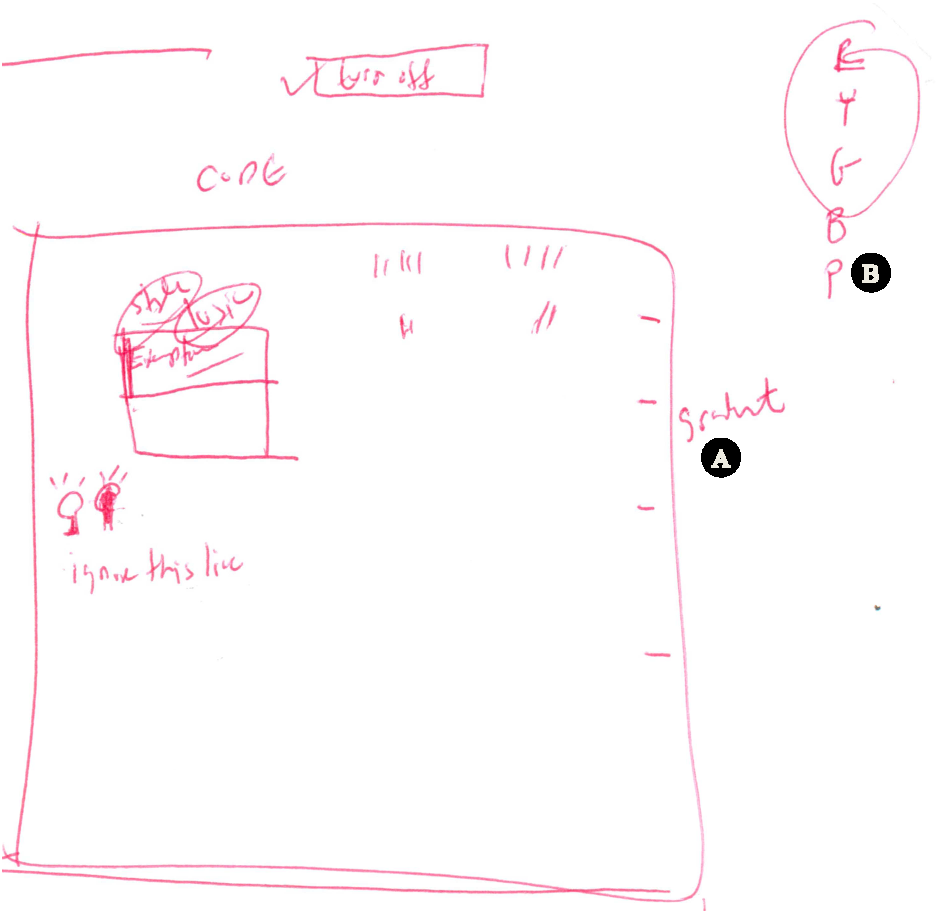
\includegraphics[width=\textwidth]{figs/participatory.pdf}
	\caption{One participant's participatory design drawing; (A) shows where Matt wants the gradient colors and (B) shows the way his current tool represents severity.}
	\label{fig:drawing}
\end{figure}

Other suggestions made by participants throughout their sessions include having ``plastic'' editors that fold and expand to show and hide information, visual output (i.e. pie-style diagram of project and bugs in it), and using a heat map to show where the most critical bugs in a project are. One interesting suggestion was to use gradient colors instead of multiple different colors to represent defect severity. Figure~\ref{fig:drawing} shows one of the drawings completed by a participant during participatory design; he labeled the side of the editor ``gradient'' (A) where he would like to see his severity representation. In the top right corner, Matt also lists the colors that his current tool uses (B); for example, ``R'' means red. The idea behind this is not new; other studies have focused their attention on effectively using colors for error representation~\cite{Oberg:1992:Gradients,Murphy-Hill:2010:Ambient}.



\subsection{Why do developers have difficulty interpreting tool notifications? [Challenges]}\label{subsec:s2}
% session study (completed)
\subsubsection{Study rationale.} Program analysis tools, such as static analysis tools, refactoring tools, and code smell detectors, can ease manual and sometimes tedious software development tasks by automatically analyzing and modifying source code~\cite{adolph2011using,Murphy-Hill:2010:Ambient}. 
Output from these tools, such as warnings and errors, come in the form of textual or visual notifications that vary from tool to tool.
In our previous interviews, 20 professional developers reported not using static analysis tools, one type of program analysis tool, because notifications can be difficult to interpret~\cite{johnson2013don}. The goal of this study was to understand what makes it challenging for developers to interpret program analysis tool notifications. To identify challenges, we examined tool use through the lens of communication theory~\cite{bowman1987modeling}. 

\subsubsection{Research questions.}

\begin{labeling}{questions}
	\item [RQ1] Why do developers encounter challenges when interpreting program analysis tool notifications? 
\end{labeling}

Using Hannay and colleagues' guidelines~\cite{hannay2007systematic}, I framed the question as \emph{why} rather than \emph{what} to support building a theory that explains the challenges developers encounter.

\subsubsection{Participants.}


\subsubsection{Methodology.} To answer my research question, I observed participants while using three different program analysis tools.

\vspace{0.5em}
\noindent\textit{Program Analysis Tools Investigated.}
My research currently focuses on tools that can be used in the Eclipse Integrated Development Environment (IDE)~\cite{EclipseIDE}. I chose Eclipse because it is one of the most widely used IDEs~\cite{Goth:2005:Beware}, making it easier to recruit qualified participants, and because it is compatible with a variety of tools. I selected FindBugs, the Eclipse Java Compiler, and
EclEmma as mature, popular tools.

\begin{figure} [h]
	
	\subfigcapskip = 1pt
	\subfigure[Source Code]{
		\fcolorbox{lightgray}{white}{\parbox{\dimexpr\linewidth-2\fboxsep-2\fboxrule}{
				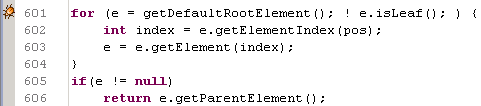
\includegraphics[width =3.3in] {figs/N4(no_tooltip)}
			}}
			\label{fig:N4code}
		}
		
		%The space between the figure and the caption
		\subfigcapskip = 1pt
		\subfigure[Short Description]{
			%From http://tex.stackexchange.com/questions/120530/wrapping-text-inside-framebox
			%\framebox (or fcolorbox) makes the box around the text.  The \parbox allows for wrapping
			%The \dimexpr stuff makes it fit in the column.  You don't need manual
			\fcolorbox{lightgray}{white}{\parbox{\dimexpr\linewidth-2\fboxsep-2\fboxrule}{
					{\scalebox{.8}{Nullcheck of e at line 605 of value previously dereferenced in \texttt{javax.-}} \\
						\scalebox{.8}{\texttt{swing.text.DefaultStyledDocument.getParagraphElement(int)} } \\
					}
					
					\label{fig:N4tooltip}
				}}
			}
			\subfigcapskip = 1pt
			\subfigure[Full Description]{
				\fcolorbox{lightgray}{white}{\parbox{\dimexpr\linewidth-2\fboxsep-2\fboxrule}{
						
						{\scalebox{.8}{A value is checked here to see whether it is null, but this value can't} \\
							\scalebox{.8}{be null because it was previously dereferenced and if it were null a null} \\ 
							\scalebox{.8}{pointer exception would have occurred at the earlier dereference.} \\ 
							\scalebox{.8}{Essentially, this code and the previous dereference disagree as to} \\ 
							\scalebox{.8}{whether this value is allowed to be	null. Either the check is redundant} \\ 
							\scalebox{.8}{or the previous dereference is erroneous.} 
						}
						
						\label{fig:N4full}
					}}
				}
				\caption{A notification of a previous null check from FindBugs (FB4).}
				\label{fig:N4}
			\end{figure}

\textsc{FindBugs (version 2.0)} notifications communicate with the developer about defects in her
code based on code patterns. Bug icons (
\includegraphics[height=9px]{figs/bug}) in the gutter are colored red
to indicate the ``scariest'' code patterns, orange for ``scary'' patterns, yellow
for ``troubling'' patterns, and blue for ``of concern.'' Text descriptions are
available by hovering over or clicking the 
\includegraphics[height=9px]{figs/bug} icon as seen in Figure~\ref{fig:N4}.


\begin{figure} [h]
	\subfigcapskip = 1pt
	\centering
	\subfigure[Source Code]{
		\fcolorbox{lightgray}{white}{\parbox{\dimexpr\linewidth-2\fboxsep-2\fboxrule}{
				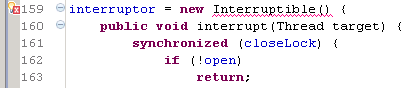
\includegraphics[width=2.6in]{figs/comp-notification}
				\label{Compcode}
			}}}
			\subfigcapskip = 1pt
			\subfigure[Text Description]{
				\fcolorbox{lightgray}{white}{\parbox{\dimexpr\linewidth-2\fboxsep-2\fboxrule}{
						
						{\scalebox{.8}{The type \texttt{new AbstractInterrruptibleChannelInterruptible()} } \\
							\scalebox{.8}{must implement the inherited abstract method \texttt{new AbstractInterr-}} \\ 
							\scalebox{.8}{\texttt{uptibleChannel.Interruptible.interrupt()}}
						}
						
						\label{Comptext}
					}} }
					
					\caption{An Eclipse compiler notification about unimplemented methods (CMP5).}
					\label{fig:notificationCOMP} 
				\end{figure}

\textsc{Eclipse Java compiler (JDT version 3.8)} notifications communicate with developers when their program cannot
compile and provide warnings about suspicious code~\cite{EclipseCompiler}.
Notifications are typically shown as squiggly underlines in the editor. Like FindBugs, the compiler uses color to represent severity; errors
are shown as red underlines, warnings as yellow underlines.
Underlines are augmented with gutter icons
(
\includegraphics[height=9px]{figs/comp-x}), as shown in
Figure~\ref{fig:notificationCOMP} at line 159. When the developer mouses over
the underlined code or the 
\includegraphics[height=9px]{figs/comp-x} icon, the
notification displays a text description (Figure~\ref{Comptext}). Unlike FindBugs, clicking the gutter icon does not provide a detailed description. Instead, clicking the icon provides possible fixes that can be automatically applied to the code called quick fixes.

\begin{figure} [h]
	\subfigcapskip = 1pt
	\centering
	\subfigure [Source Code with Highlighting]{ 
		\fcolorbox{lightgray}{white}{\parbox{\dimexpr\linewidth-2\fboxsep-2\fboxrule}{
				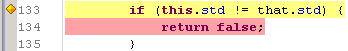
\includegraphics[width=2.3in]{figs/EclExample}
				\label{ECLcode}
			}}}
			\subfigcapskip = 1pt
			\subfigure[Text Description]{
				\fcolorbox{lightgray}{white}{\parbox{\dimexpr\linewidth-2\fboxsep-2\fboxrule}{
						\centering
						{\small ~~~1 of 2 branches missed~~~ }
						\label{Ecltext}
					}}
				}
				
				\caption{An EclEmma notification about partial branch coverage (ECL3).}
				\label{fig:notificationECL}
			\end{figure} 

\textsc{EclEmma (v2.2)} is a code coverage tool that executes a program, typically with JUnit
as the driver~\cite{JUnit}, to communicate with the developer about code paths that did and
did not get exercised. EclEmma uses highlighting to indicate code execution; code highlighted in
green was executed, red was not executed, and yellow was partially executed.
Figure~\ref{fig:notificationECL} shows an example of coverage reported by
EclEmma on an \texttt{if} statement. When the developer mouses over the

\includegraphics[height=9px]{figs/diamond} icon, the tool notifies her of how many
paths got executed on the associated branch statement at line 133
(Figure~\ref{Ecltext}).

\vspace{0.5em}
\noindent\textit{Study Protocol.} 
Participants engaged with each tool I investigated during sessions that each lasted approximately one hour. Each session consisted of seventeen tasks.
I found source code for the tasks came from Sun JDK~\cite{SunJDK} and JFreeChart~\cite{JFreeChart}. I chose Sun JDK because it has a large code base from which I could easily find bugs using their publicly available FindBugs cloud report~\cite{FindBugsCloud}. I chose JFreeChart because it is a large code base with working JUnit test cases that exhibit less-than-perfect code coverage.

For each task, I presented participants with and asked them to interpret one or more notifications from each tool.
I disallowed the use of a web browser to isolate the challenges developers encounter to the notifications used by the tools and to exclude challenges caused by outside tools.
I also wanted to see if developers could interpret tool notifications without the aid of web resources. During many tasks, and at least once for every participant, participants
discussed or completed notification resolution. I did not require them to do so, since it would be unfair to ask them to resolve a notification if they did not understand it.
As participants explained the notifications, I asked follow-up questions as necessary. 


For each task, I chose notifications to represent the types of notifications developers may encounter when programming.
For FindBugs and the Eclipse compiler, I chose notifications that appeared frequently in the Sun JDK project. I chose EclEmma notifications from JFreeChart to exercise a range of its coverage scenarios. Because EclEmma's documentation does not specify the range of notifications it uses, I manually went through JFreeChart's codebase after running the tool and took note of each new coverage scenario encountered. I then included an example of each coverage scenario in the EclEmma tasks.

\begin{figure} [h]
	\subfigcapskip = 1pt
	\centering
	\subfigure[Source Code]{
		\fcolorbox{lightgray}{white}{\parbox{\dimexpr\linewidth-2\fboxsep-2\fboxrule}{
				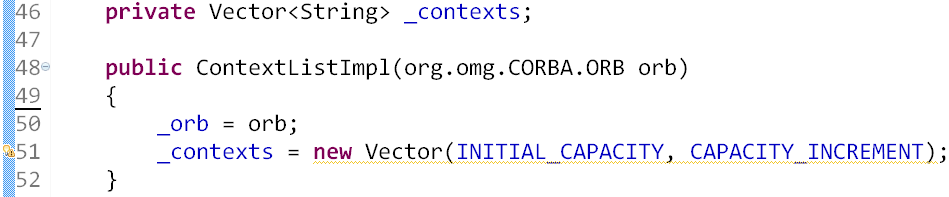
\includegraphics[width=3in]{figs/CMP2}
				\label{Comp2code}
			}}}
			\subfigcapskip = 1pt
			\subfigure[Text Description]{
				\fcolorbox{lightgray}{white}{\parbox{\dimexpr\linewidth-2\fboxsep-2\fboxrule}{
						
						{\scalebox{.8}{- Type safety: The expression of type Vector needs unchecked conversion}\\
							\scalebox{.8}{to conform to Vector<String>.} \\
							\scalebox{.8}{- Vector is a raw type. References to generic type Vector<E> }\\
							\scalebox{.8}{should be parameterized.}
						}
						
						\label{Comp2text}
					}} }
					
					\caption{A notification from the compiler about generics (CMP2).}
					\label{fig:CMP2} 
\end{figure}

For FindBugs, each task during the session corresponded to a single notification.
All but one compiler task corresponded to a single notification; because the two notifications on CMP2 (Figure~\ref{fig:CMP2}) contribute to the same problem on the same line, we presented them as one task. 
Each EclEmma task consisted of participants explaining coverage notifications for the entire class. 

\vspace{0.5em}
\noindent\textit{Data Collection \& Analysis.}
I transcribed each session and included descriptions of actions that a participant performed relevant to interpreting the notification. 
For example, if a participant navigated to different parts of the code but did not explicitly describe it, I added a description of that navigation to the transcript.


I analyzed each transcript using selective coding~\cite{corbin2014basics} to discover the challenges participants encountered with the goal of explaining the challenges programmers encounter. 
To identify a challenge in the context of my research goal, I needed concrete coding criteria. I propose that tool use is a form of communication, and therefore that challenges when interpreting a notification can be seen as miscommunication. Following this logic, I used Mustajoki's proposed model of (mis)communication to determine when a miscommunication-related challenge occurred~\cite{mustajoki2008modelling} by creating three criteria to identify a challenge: 1) the participant explicitly states a challenge, 2) is unable to explain the notification, or 3) has to take steps, outside of reading the notification, to deduce the problem.
Whether an observation met a criterion is independent of whether the participant was able to explain the notification.

The coding process was completed by two researchers, myself and a co-author on the submitted work, and in two phases. In phase 1, we each coded all the transcripts individually using the criteria above. In phase 2, we reconvened to merge our codes and check for disagreements. Of the 404 codes we originally extracted, we disagreed on 82 (20\%). 
To resolve our disagreements, we referred to our criteria; if we could not come to an agreement regarding the code fitting the criteria, we removed the statement from our data set. For four sessions, we had no disagreement.
In the end, we identified 322 codes. I put each code onto a note card, along with the participant and tool being used. 

Using the note cards created during the coding process, I completed a card sort using a methodology similar to that of Mu\c{s}lu and colleagues~\cite{Muslu:2014:Transition}. 
The goal of this card sort was to identify themes based on our codes. 
I completed the card sort with four other researchers (also co-authors on the submitted work) and in three phases.
In phase 1, we sorted all cards into high-level themes; each card could only go in one theme. 
Phase 2 focused on determining where high-level themes could be broken down into lower-level themes.
In phase 3, we focused on making sure that each card was in the best fitting theme. During this phase, we also clarified theme definitions and made note of example statements to represent each theme.

Because one my criteria is participant inability to explain a notification, any actions or statements made surrounding that occurrence was included in the card sort. Upon reflection, some emergent themes took the form of consequences of being unable to explain rather than challenges that led to inability to explain, such as notification resolution without understanding and lack of trust in the tool, therefore I will not discuss them in relation to this study. I likewise do not discuss the emergent theme of tool feature requests.

\def\toggle{
	\begin{scope}[ocg={name=test1, ref=t1, status=visible}]
		\node[inner sep=0pt] (svgPDF) at (0,0)
		{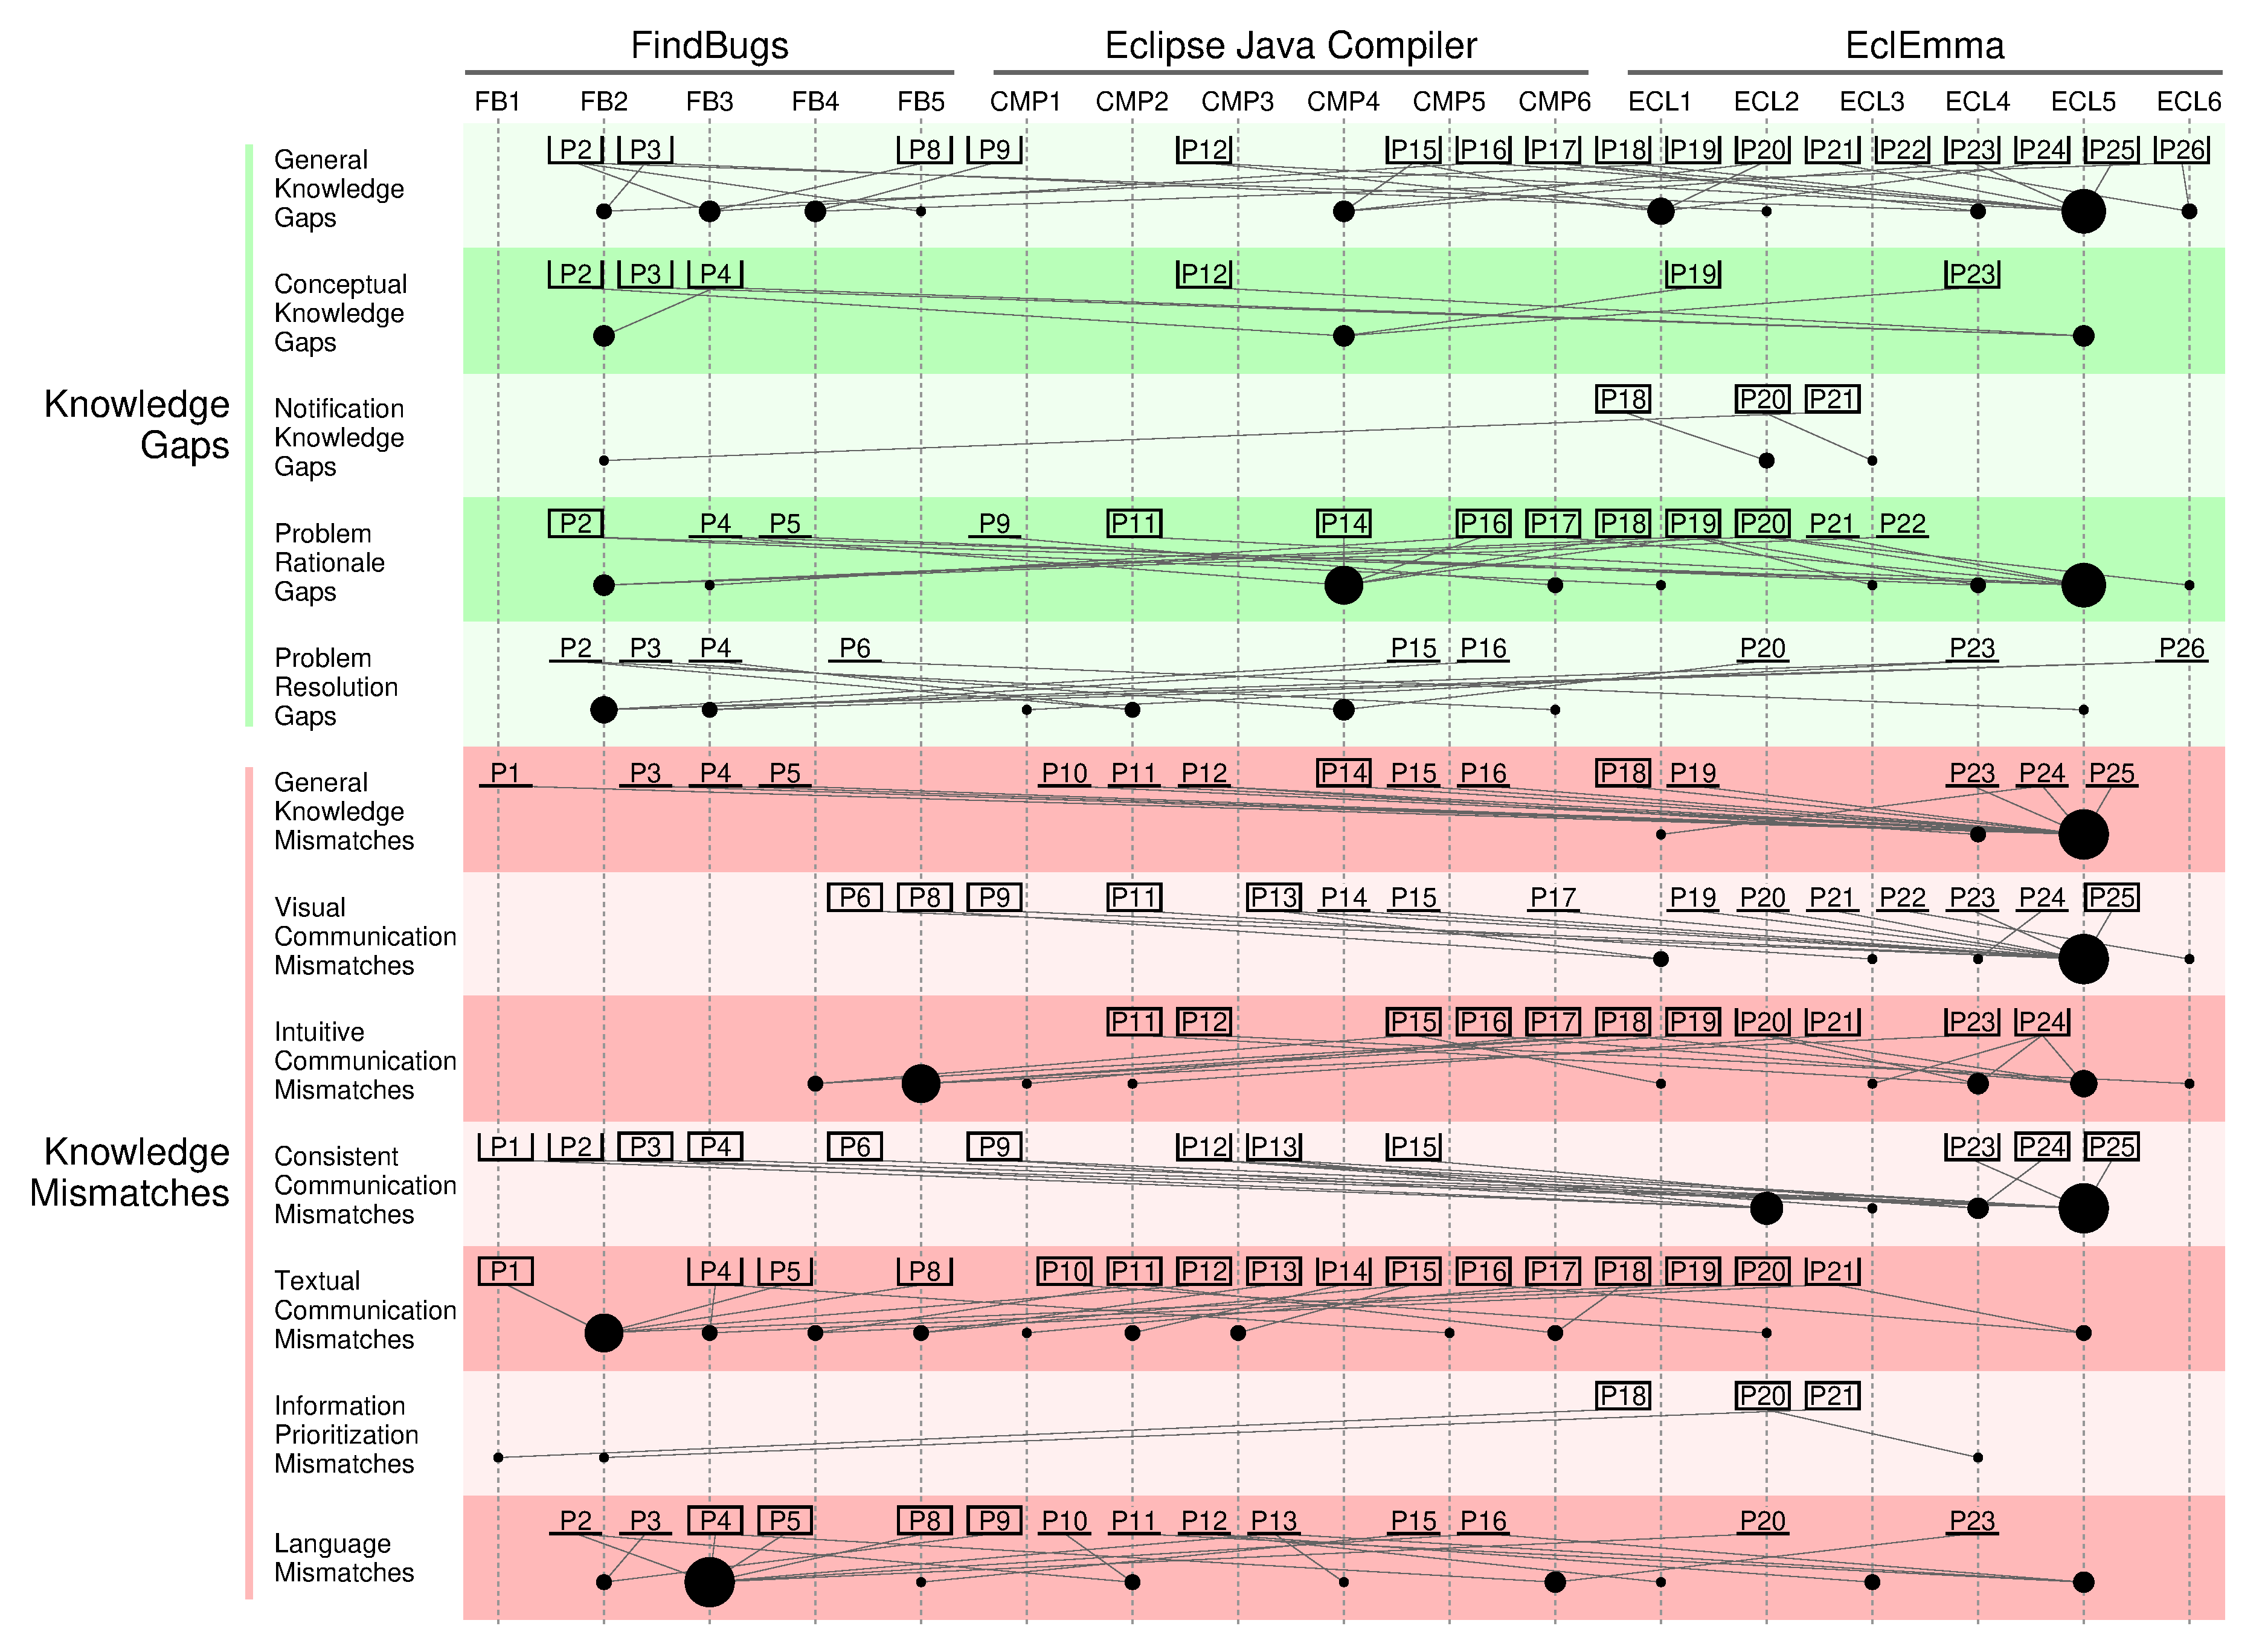
\includegraphics[width=\textwidth]{figs/Issues_Full_12.pdf}};
	\end{scope}
	\begin{scope}[ocg={name=test2, ref=t2, status=invisible}]
		\node[inner sep=0pt] (svgPDF) at (0,0)
		{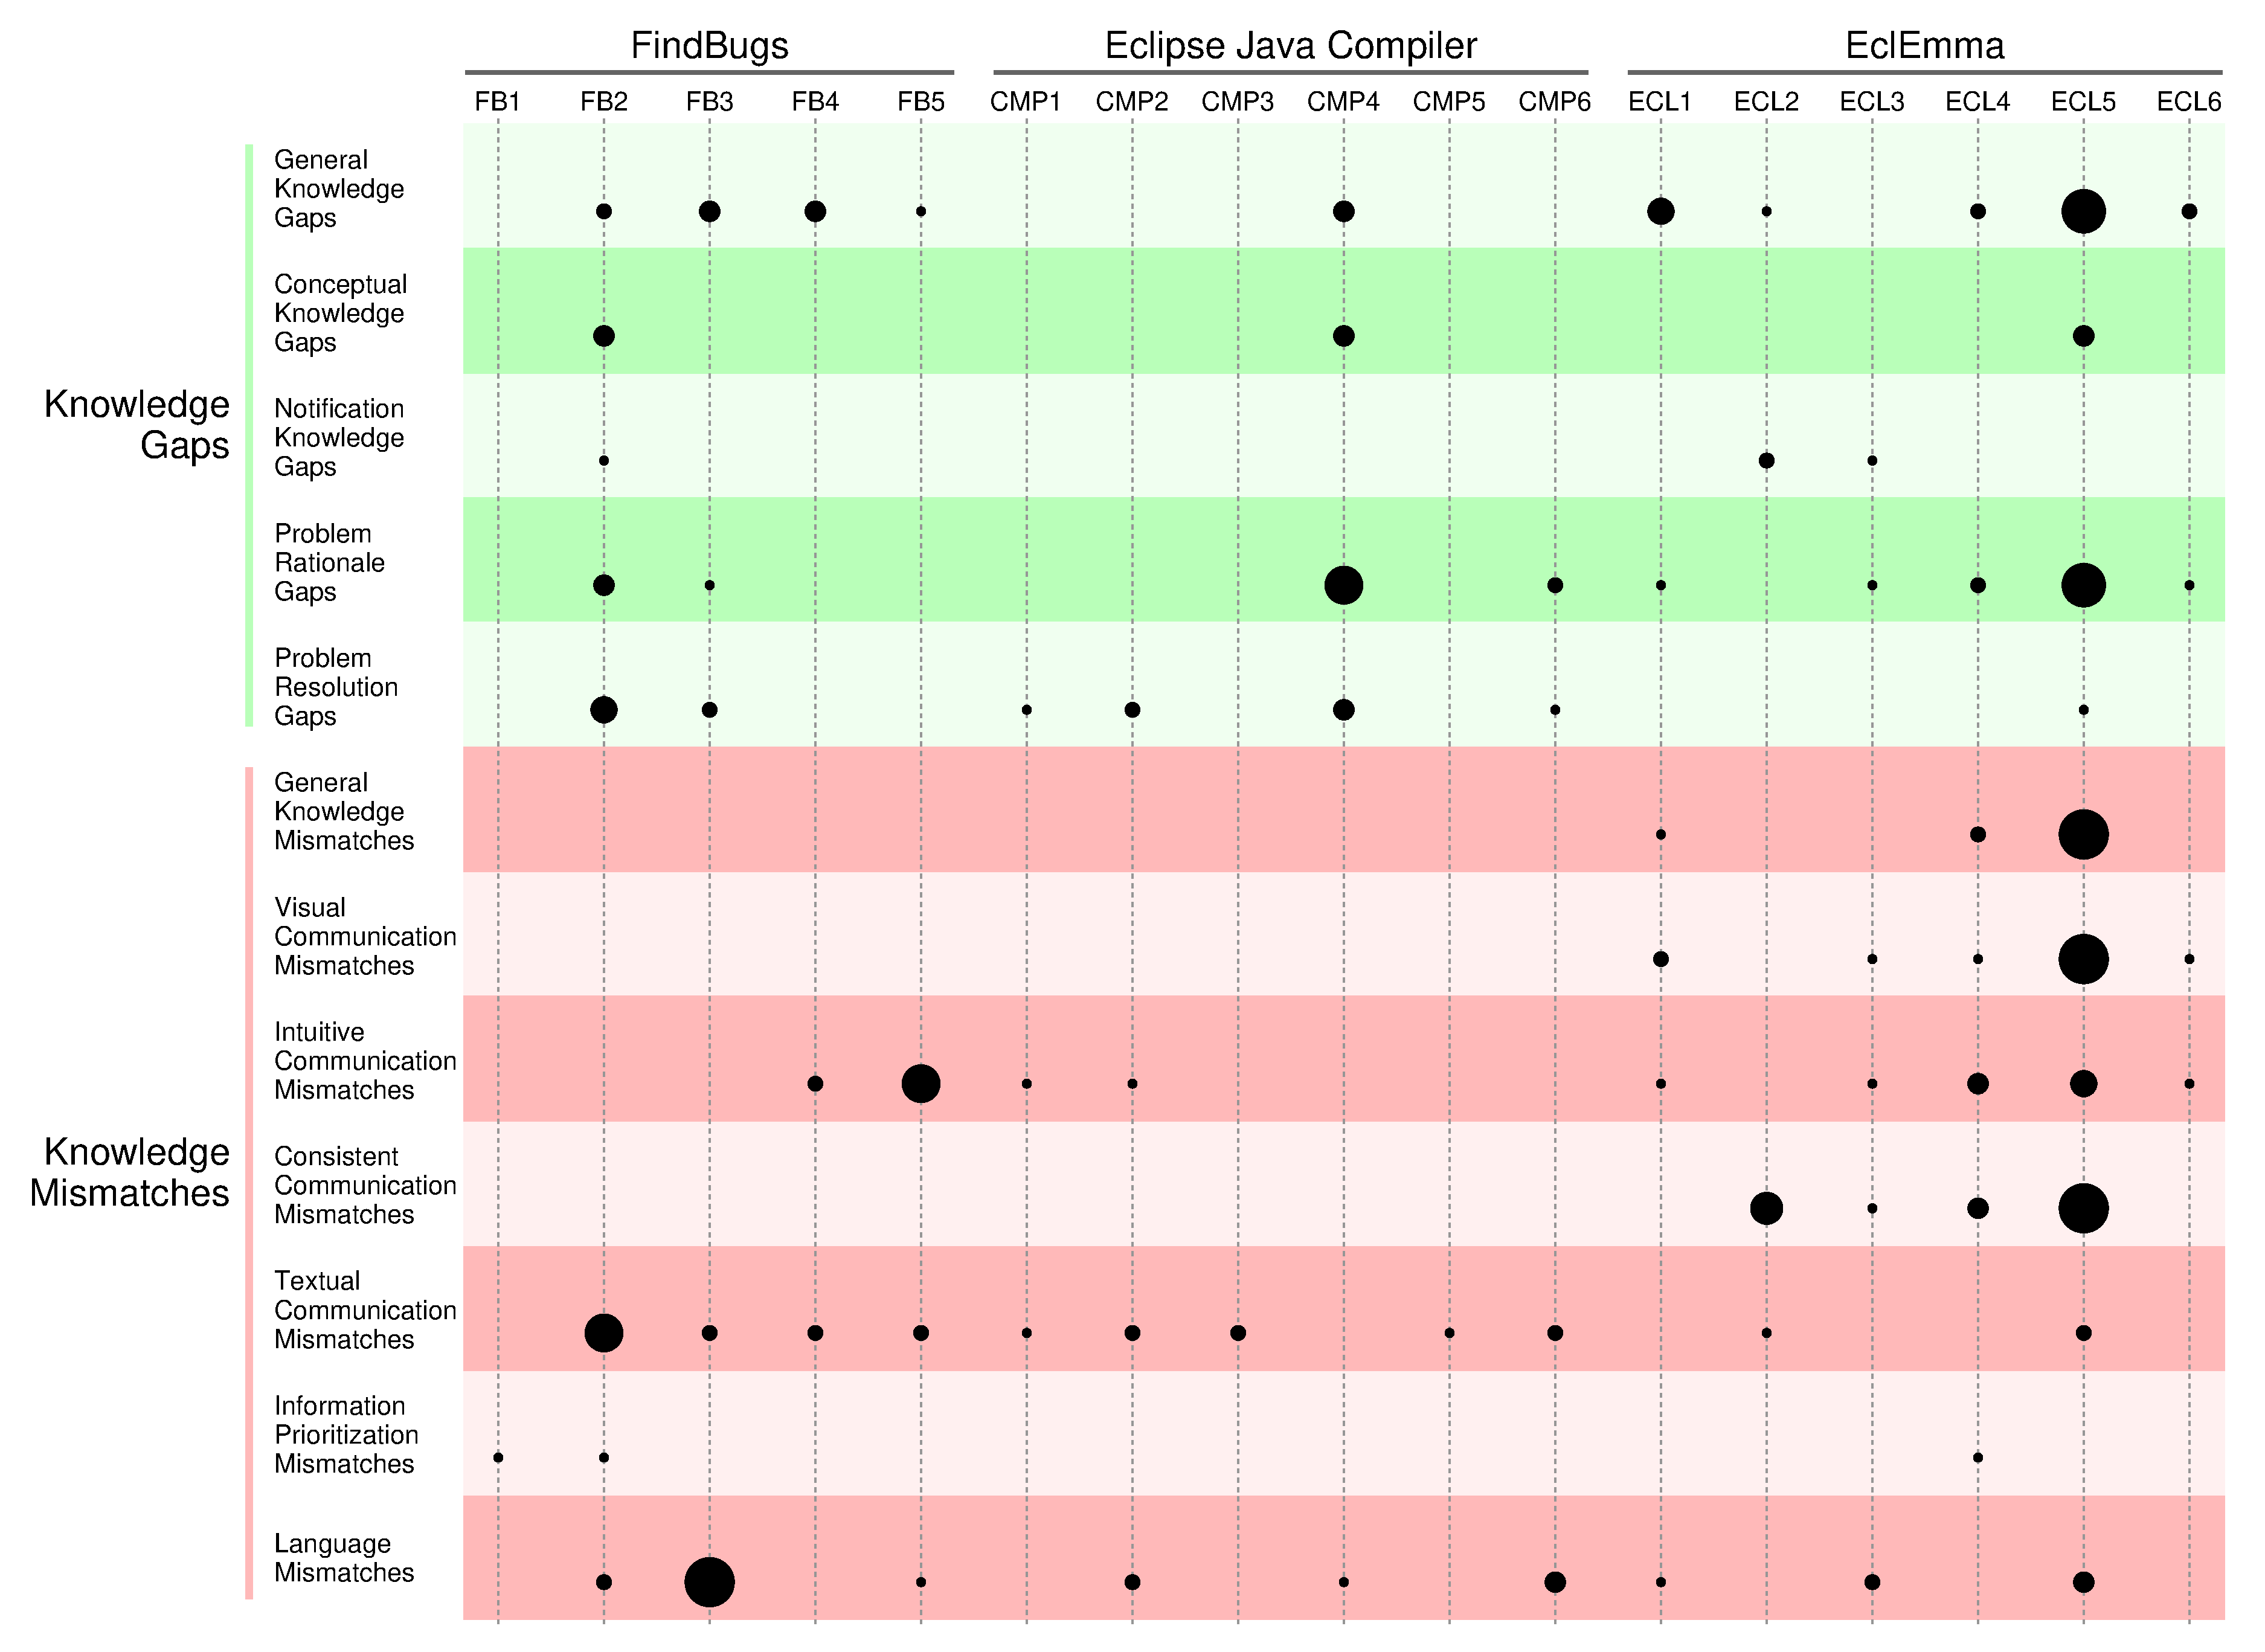
\includegraphics[width=\textwidth]{figs/Issues_Challenges_12.pdf}};
	\end{scope}
	\node[draw,switch ocg={t1 t2}] at (0,-5) {Hide/Display Details};
}

\begin{figure*}[ht]
	\centering
	\begin{tikzpicture}
	\toggle
	\end{tikzpicture}
	\caption{Distribution of challenges encountered and notifications that caused them.}
	\label{fig:results}
\end{figure*}

\subsubsection{Results.} 
I discussed my proposed theory for tool miscommunication in Section~\ref{sec:theory}; as a reminder, the theory is summarized as:

\begin{quotation}
	\noindent
	\emph{The challenges developers encounter when interpreting program analysis tool notifications are caused by gaps and mismatches between developer knowledge and how notifications communicate information.}
\end{quotation}

This theory is based on the challenges encountered by participants in this study, which are shown in  Figure~\ref{fig:results}.\footnote{Credit for the creation of this figure goes to Sarah Elder, a co-author on this work.}
Vertical lines represent the tasks and the horizontal bars indicate challenges.
The different size dots indicate how many participants encountered challenges with that notification in that theme. 
The smallest dot represents one developer and the largest dot represents eight or more developers.
Diagonal lines map participants to the challenges interpreting that notification.
\setlength\fboxsep{1pt}
When opened in Adobe Acrobat, clicking \framebox{``Hide/Display Details''} 
interactively toggles between showing and hiding this mapping.

% model building (completed)
\subsection{Can we use developer experience to predict knowledge? [Predictions]}\label{subsec:s3}

\subsubsection{Study rationale.}
In the study outlined in Section~\ref{subsec:s2}, I found that the challenges developers encounter may be due to the fact that, despite developer differences in background and knowledge, tools use the same notifications to communicate to all developers. 
I propose that communication between notifications and developers can be improved if the notifications could adapt to the developer based on the developer's knowledge of programming concepts.
This proposition is based on constructivism, a verbal communication theory that suggests awareness of how the audience might react to a message improves communication~\cite{griffin2011first}. For this to be possible in the context of tool use, tools need a way of knowing what concepts the developer knows and does not know. 
We propose using concept inventories, a method used in education research for assessing conceptual knowledge~\cite{tew2010assessing}, and the possibility of providing knowledge information to tools in the form of concept knowledge models. 
The goal of this study was to develop and assess an approach for developing models that predict knowledge of programming concepts that appear in tool notifications based on concept-specific code the developer has written. 
%We designed a concept inventory to assess conceptual knowledge and collected source code relevant to the Java concept of generics from 24 developers. We used unsupervised learning to determine a model that accurately predicts developer knowledge.
%The main contributions of this paper are: 1) an approach for assessing developer conceptual knowledge using concept inventories and 2) an approach for modeling developer conceptual knowledge based on concept-specific code written by a given developer.

\subsubsection{Hypotheses.}

\begin{labeling}{hypotheses}
	\item [H\textsubscript{1}] We can predict conceptual knowledge using source code as a primary source of developer data.
	\item [H\textsubscript{2}] Concept-specific code increases model accuracy and precision compared to a model that uses lines of code (LOC) only.
\end{labeling}

\subsubsection{Approach.}
\vspace{0.5em}
\noindent\textit{Assessing \& Encapsulating Conceptual Knowledge.}
To assess \& encapsulate developer knowledge as the dependent variable my our models, I borrowed from computer science education literature and developed a concept inventory~\cite{tew2010assessing}. 
To determine the questions for the inventory, I identified key generics concepts. I used the Oracle Java Tutorial on Generics\footnote{\url{http://docs.oracle.com/javase/tutorial/java/generics/}} to find and map the relationships between generics concepts and ancestor concepts; if Lesson 5 built on top of Lesson 1, I considered Lesson 5 an ancestor of Lesson 1. For example, based on the generics tutorial, I labeled Upper Bounded Wildcards as an ancestor concept to Wildcards. Once I had the key concepts, I mapped each level of Bloom's Taxonomy to at least one key concept. From this process, I derived 11 questions.

Next, to test the validity of our concept inventory, I used item and distractor analysis in R. Item analysis determined if the items on our inventory contribute are valid methods of assessment; from this process we eliminated 1 question, which gave us a final set of 10 questions.  Distractor analysis determined if the options provided for a given question are fair and if the incorrect options contribute to the quality of our inventory; because each option was selected at least once for each inventory item, and most often the correct option was chosen, I kept all response options for each inventory item.

For additional validation and reliability assessment, I added a self--reporting question that asks developer ``On a scale of 1 to 10, 1 being little to no knowledge, how would you score your knowledge of Java generics?'' 
By decreasing the spread of rank values for a developer to consider when deciding which value best represents how much they know, we increase the potential for accurate self-reports. To simplify the process of comparing self-reports to actual score each question is worth 1 point, making the maximum score a 10 to match the maximum possible self-report value. 
Examining the 65 responses on the inventory to date, self-report scores matched actual score 18\% of the time (12 out of 65). Most often (35 out of 65) developers estimated their knowledge within 1--2 points of their actual score. This suggests that along with objectively evaluating understanding, our concept inventory yields scores that map to how much developers think they know.

\vspace{0.5em}
\noindent\textit{Source Code Analysis.}
To test my hypotheses, I chose Java generics as the initial concept. I made this decision primarily because generics requires motivation on behalf of the developer to explore beyond the basics and is a concept appears in notifications across program analysis tools. When we say motivation, we refer to an intrinsic motivation to learn that stems from an interest in learning~\cite{krapp1999interest,hall2008we}.		
Another advantage to using a concept like generics to test my hypotheses is that it is multi-faceted; there are enough features of and ways to use generics for there to be relationships that I can explore and use to generalize for applicability to other concepts.

To determine the independent variables for my model, I analyzed for code contributions and assigned them to developers using version control. 
I built a Java source code analyzer that analyzes code bases for concept-specific code using the Eclipse JDT ASTParser. 
One example of generics-specific code is a generic type declaration ((\texttt{public class <T> Box})).
Analyzing static code with the ASTParser detects the presence of concept-specific code, however, it cannot provide who contributed that code. 	
Therefore, I used code bases in repositories so I could determine what developer made what contribution via the commit history. 
I chose the versioning platform Git\footnote{\url{https://git-scm.com/}} so we could use JGit,\footnote{\url{http://eclipse.org/jgit/}} which allows for manipulation of Git repositories via Java code, along with ASTParser to analyze for developer code contributions.
%GitHub is a social coding website where developers can create and maintain coding projects using Git version control.\footnote{http://github.com} I chose GitHub as the first source of data for a number of reasons: 1) most repositories on GitHub are public, so I can recruit participants directly, 2) I wrote my analyzer in Java and used a JGit library that allows for manipulation of GitHub repositories via Java code, and 3) next to SVN, Git is one of the most popular versioning software in use today.\footnote{http://www.openhub.net/repositories/compare}

To test H\textsubscript{1} and H\textsubscript{2}, I collected concept-specific code and manually collected LOC added from GitHub, a social coding site where developers can create and maintain Git repositories.\footnote{\url{http://www.github.com}} To determine LOC, I manually checked the contributions reported by GitHub for each developer's repositories. To determine what concept-specific code to analyze for, I used the same key concepts identified for the concept inventory (i.e. generic type declarations). I collected 11 different types of generics usage, such as generic type declarations and usage of the Wildcard (\texttt{?}) generic type.\footnote{The repository that holds our analyzer can be found at \url{https://github.com/brittjay0104/APATIANproto.git}.}

Analyses I have completed towards the idea of adapting tool notifications suggest time may play a factor in how predictive code contributions are~\cite{johnson2015bespoke}, therefore we also used version control to detect when the most recent contribution of each type of generics usage was made.
The output of my analyzer for each repository is an occurrence count for all contributed generics code and when the most recent contribution for each type of generics.
To determine which types of generics usage might be more advanced than others, I used the output from our analyses to create a hierarchy of generics feature usage. The feature hierarchy, along with a description of the creation process and usage, can be found on-line.\footnote{http://www4.ncsu.edu/~bijohnso/docs/feature-map.pdf}

% FEATURES AND HEURISTICS
To increase the generalizability of the model to other concepts, I characterized the independent variables for the model by grouping the types of generics usage collected based on \emph{features} of the data. For example, a feature of type declarations and type parameter methods (\texttt{public <T> method()}) that groups them together is that the developer wrote new generic code for use by other developers, rather than using existing generic code.
The set of features I identified among the data are as follows:
\begin{itemize}
	\item \textbf{Declared Generics:} I computed Declared Generics by adding together counts from the types of generics where the developer wrote new generic code for use by themselves or others (i.e. type declarations).
	\item \textbf{Used Generics}: I computed Used Generics by adding together counts from the types of generics that are ways to use generics, as opposed to contributing to a new generic type (i.e. method invocations).
	\item \textbf{Levels of Generics Usage:} I computed the Levels of Generics Usage by adding together counts from the types of generics that would be considered on a basic, intermediate, or advanced level of usage. I used the feature hierarchy discussed above. 
\end{itemize}

\noindent I also defined two \emph{heuristics} to apply to the feature groups:

\begin{itemize}
	\item \textbf{Recency:} The recency heuristic takes each of the initial heuristics and multiplies each value by 1.0 if the most recent contribution was made in the last week, 0.8 if between one week and one month, 0.6 for 1--6 months, 0.4 for one year, and 0.2 for more than one year.
	For example, if, the total number of declarations made by the developer (Declaration heuristic) is 198 and the most recent declaration was written between one week and one month, the Declaration Recency (DeclRecency) heuristic value would be 158.4 (\(198 \times 0.8)\). 
	\item \textbf{Natural Log:} This heuristic calculates natural log of each feature group before and after the recency heuristic is applied.
\end{itemize}
%	we were able to build models with useful levels of precision and recall

I defined a recency heuristic because previous analyses suggest time may be a factor to consider when modeling knowledge~\cite{johnson2015bespoke}.	
I applied natural log to the data following the reasoning of Fritz and colleagues, who used natural log in their models to account for the potential for large differences in variable values~\cite{fritz2010degree}. For example, some repositories returned counts in the thousands for class instantiations but counts of zero for explicit method invocations; this might cause our model to put more weight on the contribution of feature groups and heuristics that include class instantiations than it truly contributes.
I used both the \emph{features} and \emph{heuristics} defined above to determine the independent variables for analyses.

\vspace{0.5em}
\noindent\textit{Data Analysis.} % TODO if I get more developers, would I increase this number of could those go towards the next study (scalability)? (probably depends on how many more -- can I add some to the 24 for model building/assessment but then still have some I can leave out for validation of the model?)
To define the relationship between the dependent and independent variables, I used Weka~\cite{Hall:2009:WDM:1656274.1656278} for access to machine learning algorithms suitable for my small dataset of 24 GitHub developers; only 24 developers completed the concept inventory, which was necessary for developing my current approach. 
Specifically, I used Weka's J48 classifier~\cite{witten1999weka} to create decision trees.

To select the independent variables best suited for the model, I used Correlation-based Feature Selection (CFS) in Weka. This analysis runs k-fold cross validation using the independent variables passed in; to lower the potential for a model with overestimation bias, I maintained even and sizable chunks by using 4-fold cross validation.
CFS evaluates each attribute on its predictive ability and uses cross-validation to indicate how stable the best subset of variables is based on how many folds the variable appeared in.
For increased model stability, I selected the variables that appeared in more than one fold.

\subsubsection{Results.}

\begin{table}[h]
	\centering
	\caption{Precision, Recall, and F-Score for Beginner Classification}
	\label{tab:beginner}
	\begin{tabular}{llll}
		\hline
		\multirow{2}{*}{}                                                    & \multicolumn{3}{c}{\textbf{Beginner}}                   \\ \cline{2-4} 
		& \textit{Precision} & \textit{Recall} & \textit{F-Score} \\ \hline
		\textbf{LOC}                                                         & 0.5                & 0.333           & 0.4              \\
		\textbf{DeclRecency}                                                 & 0.667              & 0.333           & 0.444            \\
		\textbf{\begin{tabular}[c]{@{}l@{}}DeclRecency +\\ LOC\end{tabular}} & 0.625              & 0.833           & 0.714       \\
		\hline    
	\end{tabular}
\end{table}

\begin{table}[h]
	\centering
	\caption{Precision, Recall, and F-Score for Intermediate Classification}
	\label{tab:intermediate}
	\begin{tabular}{llll}
		\hline
		\multirow{2}{*}{}                                                    & \multicolumn{3}{c}{\textbf{Intermediate}}               \\ \cline{2-4} 
		& \textit{Precision} & \textit{Recall} & \textit{F-Score} \\ \hline
		\textbf{LOC}                                                         & 0.636              & 0.778           & 0.7              \\
		\textbf{DeclRecency}                                                 & 0.727              & 0.889           & 0.8              \\
		\textbf{\begin{tabular}[c]{@{}l@{}}DeclRecency +\\ LOC\end{tabular}} & 0.75               & 0.667           & 0.706        \\   
		\hline
	\end{tabular}
\end{table}


\begin{table}[h]
	\centering
	\caption{Precision, Recall, and F-Score for Advanced Classification}
	\label{tab:advanced}
	\begin{tabular}{llll}
		\hline
		\multirow{2}{*}{}                                                    & \multicolumn{3}{c}{\textbf{Advanced}}                   \\ \cline{2-4} 
		& \textit{Precision} & \textit{Recall} & \textit{F-Score} \\ \hline
		\textbf{LOC}                                                         & 0.875              & 0.875           & 0.875            \\
		\textbf{DeclRecency}                                                 & 0.778              & 0.875           & 0.824            \\
		\textbf{\begin{tabular}[c]{@{}l@{}}DeclRecency +\\ LOC\end{tabular}} & 1                  & 0.875           & 0.933     \\
		\hline      
	\end{tabular}
\end{table}


\begin{table}[h]
	\centering
	\caption{Total Precision, Recall, and F-Score}
	\label{tab:total}
	\begin{tabular}{llll}
		\hline
		\multirow{2}{*}{}                                                    & \multicolumn{3}{c}{\textbf{Total}}                      \\ \cline{2-4} 
		& \textit{Precision} & \textit{Recall} & \textit{F-Score} \\ \hline
		\textbf{LOC}                                                         & 0.684              & 0.696           & 0.683            \\
		\textbf{DeclRecency}                                                 & 0.729              & 0.739           & 0.715            \\
		\textbf{\begin{tabular}[c]{@{}l@{}}DeclRecency +\\ LOC\end{tabular}} & 0.804              & 0.783           & 0.787      \\
		\hline     
	\end{tabular}
\end{table}


Based on developer classifications and the set of independent variables, CFS identified two variables that fit my variable selection criteria: LOC and DeclRecency.  	
I created three decision tree models: 1) LOC only (Figure~\ref{fig:LOC}, 2) DeclRecency only (Figure~\ref{fig:decl}, and 3) LOC \(+\) DeclRecency (Figure~\ref{fig:declLOC}. I created a model based on LOC only to test H\textsubscript{2}. 
To further explore how each affects overall model accuracy and precision for H\textsubscript{1} and H\textsubscript{2}, I created a model using both LOC and DeclRecency.
The values for each model's \emph{precision}, \emph{recall}, and \emph{F-Score} values are shown in Table~\ref{tab:beginner} (Beginner), Table~\ref{tab:intermediate} (Intermediate), Table~\ref{tab:advanced} (Advanced), and Table~\ref{tab:total} (Total).
%	We observed the model's ~\cite{olson2008advanced}; 

% H1 --> can use source code
\vspace{0.5em}

\begin{figure} [h]
	\centering
	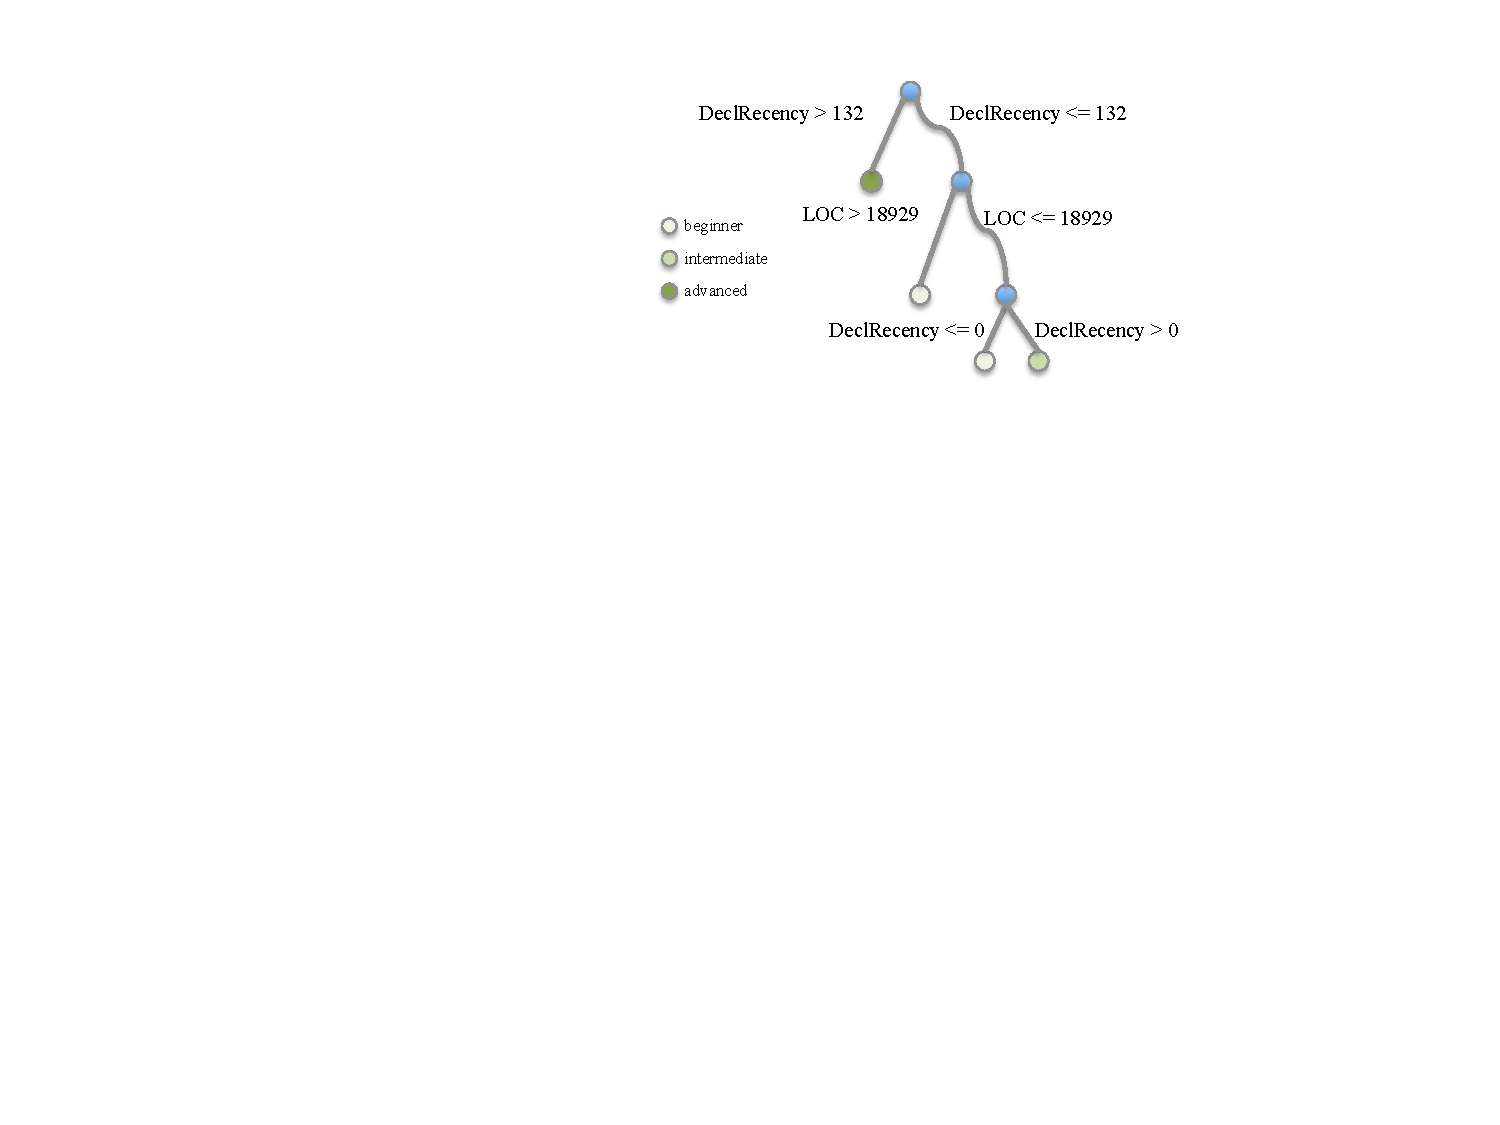
\includegraphics[width=4in]{figs/decl-LOC.pdf}
	\caption{Decision tree model using DeclRecency and LOC as independent variables.}
	\label{fig:declLOC}
\end{figure}

\begin{figure} [h]
	\centering
	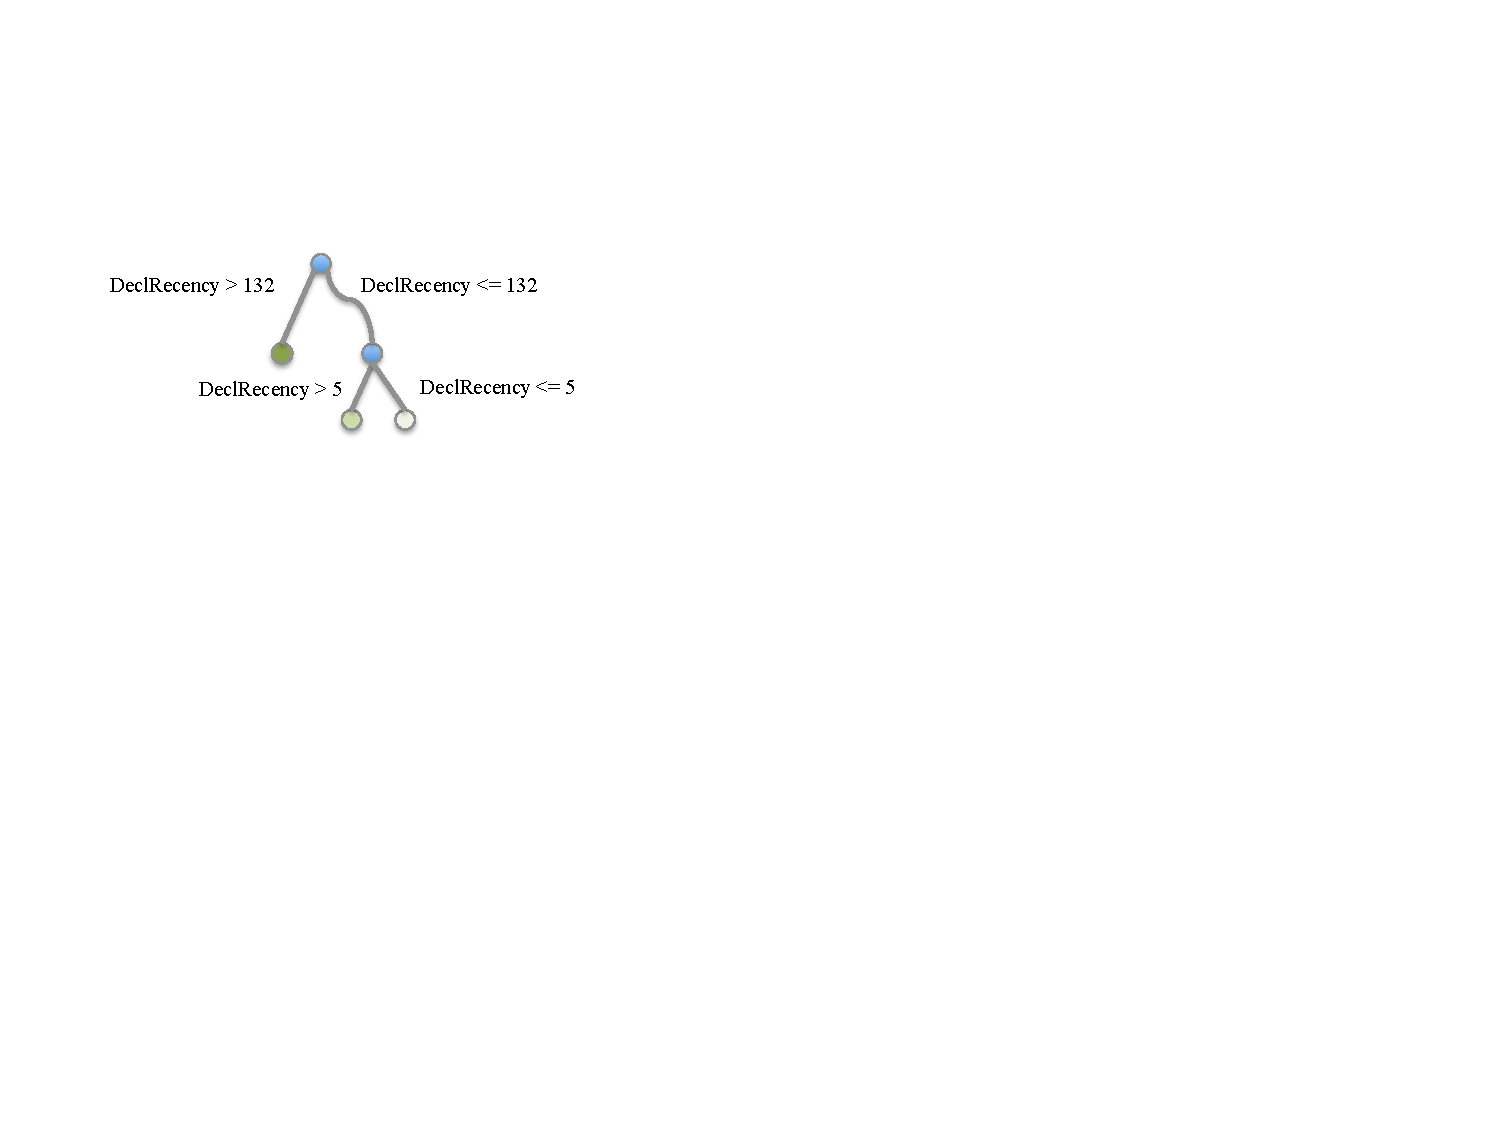
\includegraphics[width=3.5in]{figs/decl.pdf}
	\caption{Decision tree model using DeclRecency as the independent variable.}
	\label{fig:decl}
\end{figure}

\begin{figure} [h]
	\centering
	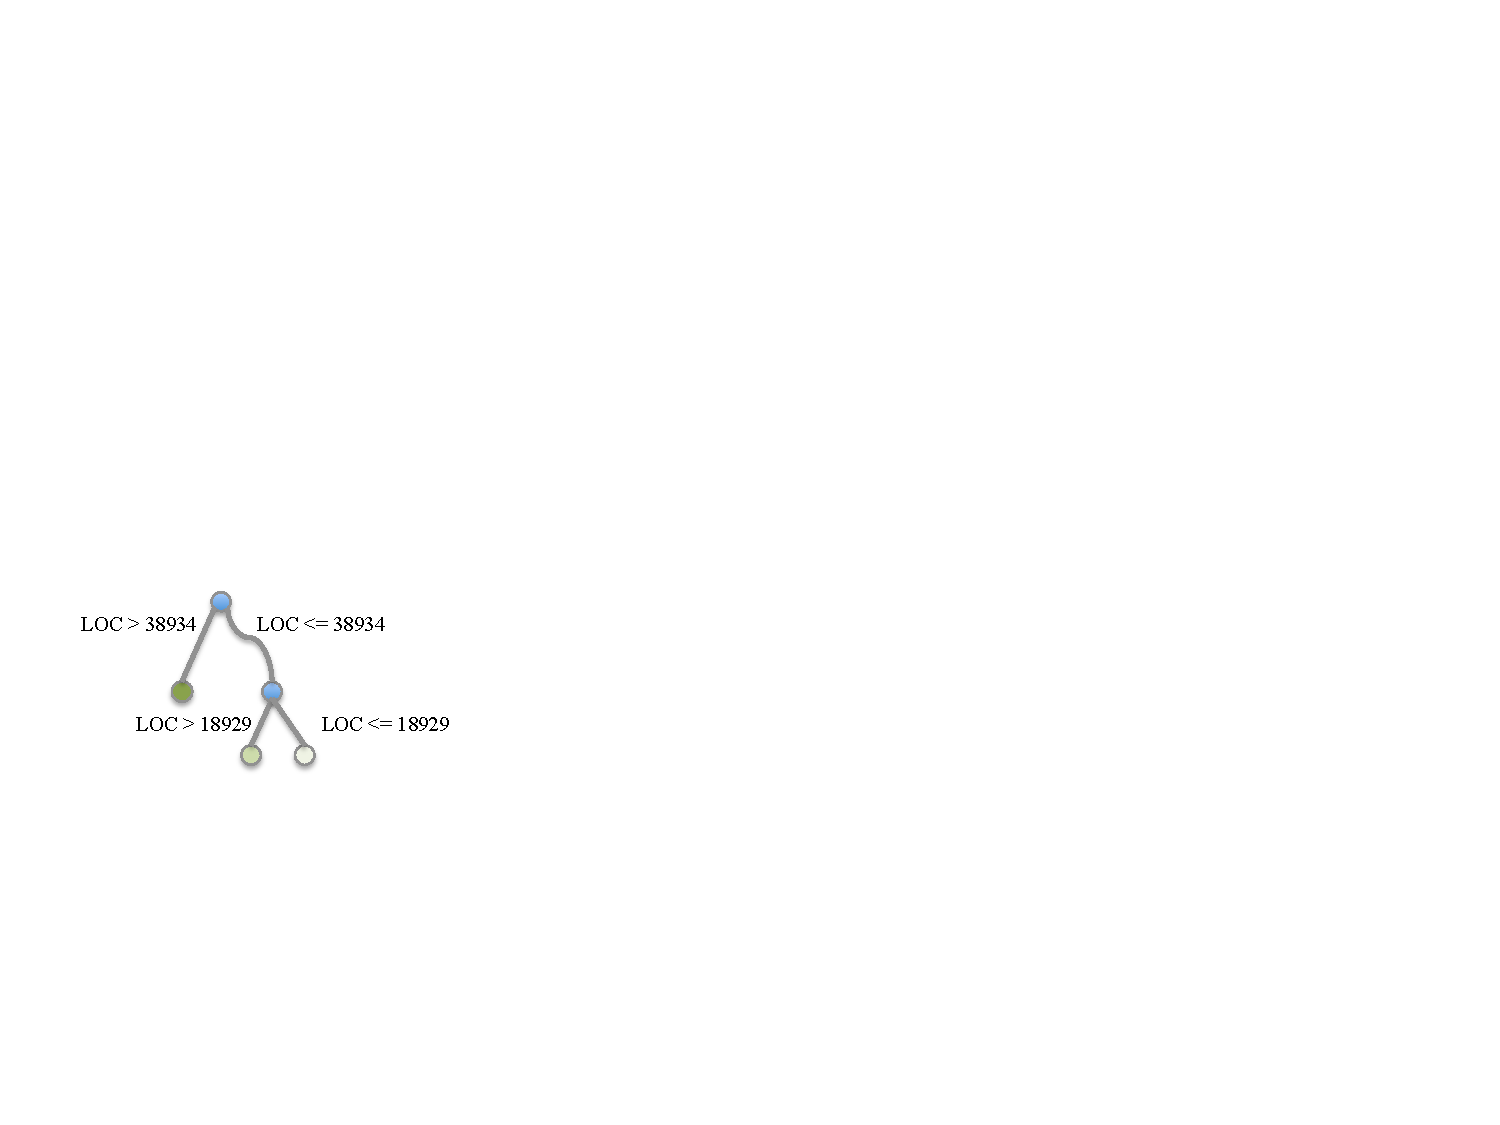
\includegraphics[width=3in]{figs/LOC.pdf}
	\caption{Decision tree model using LOC as the independent variable.}
	\label{fig:LOC}
\end{figure}

\noindent\textbf{My findings support my hypothesis that it is possible to predict conceptual knowledge using source code as a primary source of developer data. (H\textsubscript{1})}\\
All three models correctly classified developers more often than not (LOC = 70\%; DeclRecency = 74\%; Combination = 78\%); in fact, by combining LOC with DeclRecency, the accuracy of classification increased by 4\%. This increase may be due to the fact that, as existing research suggests, all experiences contribute to overall knowledge~\cite{argote2011organizational}. Similarly, general coding experience seems to also contribute to conceptual knowledge.

Based on the models shown in Figure~\ref{fig:declLOC} and Figure~\ref{fig:decl}, how recently code contributions are made also affect conceptual knowledge. Based on the recency heuristic, a higher DeclRecency value suggest more recent code contributions. This suggests that determining a developer's knowledge of concepts may require both declarations and recent experience with declarations. 


% H2 --> concept-specific code better
\vspace{0.5em}

\noindent\textbf{My findings support my hypothesis that concept-specific code improves model performance compared to a model that uses LOC only. (H\textsubscript{2})}\\
The LOC model's precision, recall, and F-Score suggest it may be better at classifying developers with advanced generics knowledge than the DeclRecency model (Figure~\ref{tab:advanced}). However, overall model accuracy is higher in the DeclRecency model (74\%) than the LOC model (70\%) (Table~\ref{tab:total}. There was also a slight performance increase overall, with increased precision and F-Score for beginner (\(+ 0.167\), \(+ 0.04\)) and intermediate (\(+ 0.09\), \(+ 0.1\)) classification and increased total precision (\(+ 0.05\)), recall (\(+ 0.04\)), and F-Score (\(+ 0.03\)). Also, as shown in Figure~\ref{fig:declLOC}, LOC only becomes relevant when classifying beginner and intermediate developers. This may be because beginner and intermediate developers do not declare enough generics to make an informed decision without some reference to general experience they have.
Regardless, these findings suggest that although both LOC and concept-specific code can both be used to predict conceptual knowledge, concept-specific code increases overall model accuracy and precision.


\subsection{Does my prototype concept knowledge model scale? [Scalability]} \label{subsec:s4}

\subsubsection{Study rationale.} Two important aspects to consider when developing a quality tool or approach are \emph{performance} and \emph{scalability}. 
Research suggests that there is an inverse relationship between performance and scalability with respect to information systems; when performance is increased, stability decreases(and vice versa)~\cite{khaddaj2004evaluation}.
My previous study found that it is possible to assess, model, and accurately predict developer knowledge regarding Java generics (performance), based on the predictions of a prototype model (M1). However, it is not obvious 1) if M1 scales to other concepts and developers and 2) if increased scalability of M1 will decrease its performance. 
The end goal is an approach that can be applied to any concept and be used to make predictions for any Java developer (scalable) while still performing at a high level. Therefore, I designed a study where I will explore the scalability of M1 to other programming concepts and different sets of developers and the affects on model performance. 

Assessing scalability in the context of a mathematical model is a primarily quantitative process. Although there is value in quantitative findings, my research experience suggests that there is a richness in qualitative data that cannot be achieved with quantitative data and analyses. I chose the variables for M1 based on quantitative data and analyses; however, it may be that there are other factors that contribute to developer concept knowledge I have not yet considered. Therefore, I also plan to explore the scalability, and approach that led to the creation, of M1 by interviewing and surveying developers. 

\subsubsection{Research questions.}

\begin{labeling}{questions}
	\item [RQ1] To what extent does M1 generalize to developers and concepts outside the set used to create the model?
	\item [RQ2] If M1 scales, is there decreased performance in the predictions it makes?
	\item [RQ3] Do developers agree with the factor (source code) used to develop M1?
\end{labeling}

\subsubsection{Proposed methodology.}
I plan to explore the scalability of, and refine, M1 by combining qualitative feedback with scalability assessments. One of my ongoing (implicit) model refinement efforts is finding more developers for building and assessing M1 and, if needed, creating and evaluating new models.

\vspace{0.5em}
\noindent\textit{Scalability Assessments.}
I built and assessed M1 using the same set of developers; one way I plan to assess the scalability of M1 to other developers (RQ1) is by making predictions with a separate set of developers. Doing so will allow me to observe the ability for M1 to scale to a wide range of developers. 
To assess the scalability of M1 in regards to other concepts, I plan to analyze participant repositories for concept-specific code pertaining to others Java concepts. 
To select the concepts for assessment, I plan to use the following criteria:
\begin{itemize}
	\item It is a concept that appears in program analysis tool notifications, particularly FindBugs which I plan to extend to assess the potential for adaptive notifications (Section~\ref{subsec:s5}).
	\item It is a concept that has a wide range of sub-concepts.
	\item It is a concept that has features that may go unused by most developers.
\end{itemize}

Rather than attempting to find an exhaustive list of concepts that fit one or more of these criteria, I plan to begin with the first criteria; FindBugs has a publicly available, and regularly updated, webpage with a list of the notifications it uses.\footnote{http://findbugs.sourceforge.net/bugDescriptions.html}
I plan to evaluate M1 on at least three additional concepts.

To determine if performance is affected by model scalability (RQ2), I will evaluate and compare performance on 1) the dataset used to create M1 and the new dataset and 2) the concept used to create M1 and the new set of concepts. 

\vspace{0.5em}

\noindent\textit{Qualitative Feedback Collection \& Analysis.}
% TODO should this be another RQ (i.e. do developers agree with the relationship between source code and knowledge)??
Another way I plan to assess the scalability of M1 is by conducting short, semi-structured interviews with developers (10--20) regarding their perceptions of source code and programming concept expertise (RQ3). Each interview will last approximately 30 minutes and will be divided into two phases: 1) their perception of the relationship between the code they write and their expertise regarding the concept and 2) their perception of the other factors that contribute to their knowledge of programming concepts.  

To determine if developers agree with using source code as a proxy for knowledge, and identify developer perceptions of what factors contribute most to their knowledge, I plan to 1) code each transcript and 2) perform content analysis in R~\cite{RSoftware} on interview transcripts. Content analysis assumes that content most frequently mentioned is the most important. In order to perform content analysis, I need well defined categories; this is where the coding process comes into play. Using a methodology similar to the one in Section~\ref{subsec:s2}, I will code each transcript for statements pertaining to their knowledge of concepts and experiences that contributed knowledge for them. 

Using the codes from the transcripts, I will perform content analysis to determine which factors developers feel contribute most to their knowledge.
To validate source code as a factor, and other factors that emerged during the interviews, I plan to administer a survey to another set of developers (50--100). Using data from the survey, I will perform various analyses using R. Findings from both the qualitative and quantitative analyses will serve to potentially confirm current model building efforts and inform future data analysis and model building efforts.


\subsection{Are adaptive, knowledge-based notifications more effective than one-size-fits-all notifications? [SmartBugs]} \label{subsec:s5}
\subsubsection{Study rationale.}
Based on findings from previous studies, I propose that communication between tools and developers can be improved if rather than using one-size-fits-all notifications, tools used knowledge-based notifications. Knowledge-based notifications would use the models I propose and refine in the studies from Section~\ref{subsec:s3} and Section~\ref{subsec:s4}. If communication theory applies directly to tool use, constructivism communication theory should also apply~\cite{griffin2011first}. Constructivism states that a speaker with awareness of how her audience will react to her message can tailor the message to the audience and therefore improve the audience's ability to understand and relate to the message. 
I have explicitly assessed the applicability of general communication theory to tool use (Section~\ref{subsec:s2}), however, I have not explicitly assessed the applicability of constructivism to notification and tool design. Therefore, the goal of this study is to assess whether knowledge-based communication, in regards to tool use, is better than one-size-fits-all communication.

\subsubsection{Research questions \& Hypothesis.}

\begin{labeling}{questions}
	\item [RQ1] How does existing notification design research map to differences in developer knowledge?
	\item [RQ2] Are there differences in notification design expectations across developers with differing knowledge?
	\item [H\textsubscript{1}] Adaptive, knowledge-based notifications are more effective than one-size-fits-all notifications.
\end{labeling}

\subsubsection{Proposed methodology.}
% TODO make sure to mention using FindBugs and why
To answer RQ1, I will perform a literature review of existing research on the design, presentation, and developer interpretation of tool notifications. The focus of this literature review will be to explore the design space of notifications and how developers with various backgrounds (i.e. novice versus expert) find and use information to understand problems in their code. For example, existing research suggests that experts more often rely on abstractions to understand problems in their code, while novices tend to focus on the literal features, such as the constructs in the source code~\cite{Weiser:1983:Representation}. Therefore, one potential design consideration for notifications for novices is to center the explanation around the source code, or parts of the source code, while for experts a consideration would be to use more abstractions. I will compile a list of related findings and map these findings to developer knowledge or expertise.

To answer RQ2, I will code the list of findings to determine 1) themes within a knowledge group and 2) how themes differ across knowledge groups. I plan to use a methodology similar to the methodology outlined in Section~\ref{subsec:s2}. Once I have these themes, I can begin to develop my approach for assessing H\textsubscript{1}. 

To assess H\textsubscript{1}, I plan to 1) assess potential knowledge-based notification adaptations and 2) implement and evaluate a tool that replaces one-size-fits-all notifications with knowledge-based notifications. 
I will first use findings from RQ1 and RQ2 to design notification templates that map to different levels of expertise; for consistency, I will attempt to use three groups as I did in the study in Section~\ref{subsec:s3}. 
% TODO this is incomplete!
Once I have a prototype notification design template...

Based on the results from my user study, I will develop a prototype tool, which I will call SmartBugs, that will adapt notification presentation based on developer knowledge. I plan to build SmartBugs on top of FindBugs because it is a mature, open source defect finding tool with a wide range of notifications that have no obvious pattern behind the information it provides in a given notification. FindBugs will serve as the baseline (one-size-fits-all) set of notifications to compare SmartBugs' notifications to (knowledge-based).

For the evaluation of SmartBugs, I will attempt to re-use the same participants from the studies in Section~\ref{subsec:s3} and Section~\ref{subsec:s4}. This will prevent the overhead of finding new participants with Git repositories and the potential overhead of asking more developers to take potentially multiple concept inventories.
As a back-up plan, I will consider using self--reported knowledge; my findings from the study in Section~\ref{subsec:s3} suggest that most often developers are aware of how much they know about a given concept.
% TODO what other way can I get knowledge? Anything lighter weight?

For the user evaluation, I will divide participants into two groups: one group will use FindBugs (FB) and the other will use SmartBugs(SB). Each group will have an equal number of developers from each classification group to ease the process of analyzing the data. All developers in the FB group will be presented with the normal notifications used by FindBugs. Developers in the SB group will be presented with notifications based on their classification and the mappings from RQ1 and RQ2.

To assess whether SmartBugs is more effective than FindBugs, I will observe 1) the ability for participants to understand and resolve each notification and 2) the time it takes for participants to understand and resolve each notification. I will measure understanding by requesting participants explain the notification aloud. I will assess the correctness of their explanations to determine whether they correctly interpreting the message; this will be my proxy for understanding. I will assess ability to resolve the notification by observing if the participant makes intentional code changes

I also plan to allow use of the web for both FindBugs and SmartBugs; this will inform future improvement efforts. For example, if a group of SmartBugs users have to go to the web, particularly if they are in the same classification, this information can be used to improve the information provided to developers in that classification.

To assess user satisfaction with SmartBugs and FindBugs notifications, I will administer a user satisfaction survey post-evaluation to gain insights into participant options of both sets of output.

% TODO really wanna put PD in here somewhere!


\section{Related Work}

There will be lots here -- just seemed like something I could put on the backburner for later drafts. :)

\section{Project Plan}
% TODO month by month (deadline driven - what papers?)

\subsection{Completed Projects \& Publications}

I have completed the following projects \& publications:
\begin{description}
	\item[Reasons] Completed Fall 2012; Publication: ICSE 2013
	\item[Challenges] Completed Fall 2015; Publication: FSE 2016 (in submission)
	\item[Predictions] Completed Spring 2016; Publication: VL/HCC 2016 (in submission)
\end{description}

\subsection{Upcoming Projects \& Publications}

I plan to complete the following projects \& publications by my defense in Spring 2017:

\begin{description}
	\item[Scalability] (in progress) \textit{Amend IRB for interviews and survey} (May 2 -- May 9); \textit{Data collection} (April 11 -- April 25); \textit{Conduct Interviews} (May 11 -- May 20); \textit{Data analysis} (May 21 -- May 28) ; \textit{Create and administer survey} (May 29 -- June 12); \textit{Survey analysis} (June 13 -- June 30); \textit{Publication}: ICSE 2017 (est. 8/28)
	\item[SmartBugs] \textit{Study IRB} (May 2 -- May 9); \textit{Literature Review} (June 6 -- June 12); \textit{Develop SmartBugs} (with aide of Master's student) (June 13 -- October 3); \textit{User Study} (October 10 -- October 21) ; \textit{Data analysis} (October 22 -- October 30); \textit{Write and edit draft} (November 1 - March 11/March 18); \textit{Publication}: FSE 2017 (est. 3/11) or VL/HCC 2017 (est. 3/18)
	\item[Dissertation] \textit{Write and edit draft} (January 1 -- May 1) ; \textit{Publication}: Thesis Document
\end{description}

%ICSE 2017

%FSE2017

%VLHCC (backup?)

% JOURNAL??

\section*{Acknowledgments}


\bibliographystyle{splncs03}
\bibliography{main.bib}

%
%\begin{thebibliography}{[MT1]}
%%
%\bibitem[CE1]{clar:eke}
%Clarke, F., Ekeland, I.:
%Nonlinear oscillations and
%boundary-value problems for Hamiltonian systems.
%Arch. Rat. Mech. Anal. 78, 315--333 (1982)
%%
%\bibitem[CE2]{clar:eke:2}
%Clarke, F., Ekeland, I.:
%Solutions p\'{e}riodiques, du
%p\'{e}riode donn\'{e}e, des \'{e}quations hamiltoniennes.
%Note CRAS Paris 287, 1013--1015 (1978)
%%
%\bibitem[MT1]{mich:tar}
%Michalek, R., Tarantello, G.:
%Subharmonic solutions with prescribed minimal
%period for nonautonomous Hamiltonian systems.
%J. Diff. Eq. 72, 28--55 (1988)
%%
%\bibitem[Ta1]{tar}
%Tarantello, G.:
%Subharmonic solutions for Hamiltonian
%systems via a $\bbbz_{p}$ pseudoindex theory.
%Annali di Matematica Pura (to appear)
%%
%\bibitem[Ra1]{rab}
%Rabinowitz, P.:
%On subharmonic solutions of a Hamiltonian system.
%Comm. Pure Appl. Math. 33, 609--633 (1980)
%\end{thebibliography}

%
\end{document}
